%Preamble Mainfile

%usenix style-------------------------------------------------------------------
\documentclass[letterpaper,twocolumn,10pt]{article}
\usepackage{usenix2019_v3}
%-------------------------------------------------------------------------------

%IEEE tyle----------------------------------------------------------------------
%\documentclass[10pt, conference, letterpaper]{IEEEtran}
% Enable Hyperrefs without ugly boxes
%\usepackage
%[pdfusetitle]
%{hyperref}
%\hypersetup{
%	hidelinks,%
%	colorlinks=true,%
%	allcolors=black,%
%	pdfstartview=Fit,%
%	breaklinks=true%
%}%
%-------------------------------------------------------------------------------


\usepackage[utf8]{inputenc}
% For R table rotating colnames
\usepackage{rotating}
\usepackage[T1]{fontenc}
\usepackage{tabularx}
\usepackage{lscape}
\usepackage{longtable}
\usepackage{rotating}
\usepackage{makecell}
% Check references for unused items
%\usepackage{refcheck}
% Used for nice quotes
\usepackage{csquotes}%
% For bigger sum signs
\usepackage{relsize}
% Used to display urls nicely %
\usepackage{url}%
% Necessary to provide the correct spacing for e.g. and i.e. %
\usepackage{xspace}%
% Useful for todos, used with \todo{<Text>} to make orange 
% boxes at the margins of the document. Use \todo[inline]{<Text>} for in-text-boxes
\usepackage{todonotes}%
% For the align-environment %
\usepackage{amsmath}%
% For the maths symbols %
\usepackage{amssymb}%
% For the maths text %
\usepackage{amstext}%
% package for multicolumn
\usepackage{multirow}
% Euro symbol %
\usepackage{eurosym}%
% Units such as percent, meters, seconds, ... %
\usepackage{siunitx}%
% For the x mark
\usepackage{pifont}%
% For fancy graphics
\usepackage{tikz}%
\usepackage{pgfplots}%
\pgfplotsset{compat=1.15}
% For the graph
\usetikzlibrary{shapes}%
% For stuff like right=of etc.
\usetikzlibrary{positioning}%
% For not-so-fancy graphics
\usepackage{graphicx}%
% For better quoting
\usepackage{csquotes}%
% For subfigures
% \usepackage{algorithm}%
% % For algorithm form
% \usepackage{algorithmic}%
% % for more pseudo code formulas
\usepackage[linesnumbered,ruled,lined]{algorithm2e}
% for more pseudo code goodness
%subfig and subfigures are deprecated!!!!!
%\usepackage[lofdepth,lotdepth]{subfig}%
% Correct Package: Used for side-by-side figures and tikz pictures
\usepackage[skip=6pt]{subcaption}
%
% TEMP for readable quotes
\usepackage[]{natbib}
% \newcommand{\ttext}[1]{\text{{\ttfamily\bfseries\slshape #1}}}
\newcommand{\ttext}[1]{\text{{#1}}}
%%% Coloring the comment as blue
\newcommand\mycommfont[1]{\footnotesize\ttfamily\textcolor{blue}{#1}}
\SetCommentSty{mycommfont}

\SetKwInput{KwInput}{Input}                % Set the Input
\SetKwInput{KwOutput}{Output}              % set the Output
% 
% For "Consolas" font of ttfamily fonts
%\usepackage{inconsolata} 
% 
% Enable correct jumping to Figures when referencing
\usepackage[all]{hypcap}%
% 
% Use package for more maths tools
\usepackage{mathtools}%
% 
% Make stargazer work
\usepackage{dcolumn}%
% 
\usepackage{array}%
%\newcolumntype{L}[1]{>{\raggedright\arraybackslash}m{#1}}%
%
%Used for acronyms
\usepackage{expl3}
\ExplSyntaxOn
\tex_let:D \c_minus_one \scan_stop:
\int_const:Nn \c_minus_one {-1}
\ExplSyntaxOff
\usepackage{acro}
%Used for fresher tables
\usepackage{booktabs}
%-----put new packages here
%Preamble command definitions%
%---Author affiliation formatting-----
\newcommand\Mark[1]{\textsuperscript{#1}}

%---Typography-----
% \newcommand*{\eg}{e.\,g.\@\xspace}%
% \newcommand*{\ie}{i.\,e.\@\xspace}%
% In english typography, there is no space between 'e.' and 'g.' etc.
% See The Art of Typographic Style for further reading
\newcommand*{\eg}{e.g.\@\xspace}%
\newcommand*{\ie}{i.e.\@\xspace}%54
\newcommand*{\wrt}{w.r.t.\@\xspace}%54
\newcommand{\xmark}{\ding{55}}%
\newcommand{\cmark}{\ding{51}}%

%---In-text references to labels-----
\newcommand{\refsec}[1]{\hyperref[#1]{Section~\ref{sec:#1}}}
\newcommand{\refequ}[1]{\hyperref[#1]{Equation~\eqref{eq:#1}}}
\newcommand{\reffig}[1]{\hyperref[#1]{Figure~\ref{fig:#1}}}
\newcommand{\reftbl}[1]{\hyperref[#1]{Table~\ref{tbl:#1}}}
\newcommand{\refass}[1]{\hyperref[#1]{Assumption~\ref{ass:#1}}}
\newcommand{\refthm}[1]{\hyperref[#1]{Theorem~\ref{thm:#1}}}
\newcommand{\reflemma}[1]{\hyperref[#1]{Lemma~\ref{lemma:#1}}}
\newcommand{\refalgo}[1]{\hyperref[#1]{Algorithm~\ref{algo:#1}}}
\newcommand{\refappendix}[1]{\hyperref[#1]{\ref{appendix:#1}}} % "Appendix~"
                                % is in renewed \thesection after \appendix

%------------------------------------------------------------------------------%
% Color schemes for color-blind readers: red/green blindness%
% [TOL, Paul: Color Schemes. SRON/EPS/TN/09-002, 29 September 2018]%
% Muted qualitative color schemes%
\definecolor{CMQBlueA}{HTML}{332288}  %indigo%
\definecolor{CMQBlueB}{HTML}{88CCEE}  %cyan%
\definecolor{CMQBlueC}{HTML}{44AA99}  %teal%
\definecolor{CMQGreenA}{HTML}{117733} %green%
\definecolor{CMQGreenB}{HTML}{999933} %olive%
\definecolor{CMQGreenC}{HTML}{DDCC77} %sand%
\definecolor{CMQRedA}{HTML}{CC6677}   %rose%
\definecolor{CMQRedB}{HTML}{882255}   %wine%
\definecolor{CMQRedC}{HTML}{AA4499}   %purple%
\definecolor{CMQGray}{HTML}{DDDDDD}   %pale gray%
%
%---R-Plot related-------------------------------------------------------%
\renewcommand{\rothead}[2][90]{\makebox[9mm][c]{\rotatebox{#1}{\makecell[c]{#2}}}}%
% ---Tiks/Pgfplot related-------------------------------------------------------%
\newcommand{\captionGlo}   {}%
\newcommand{\captionLocL}  {}%
\newcommand{\captionLocR}  {}%
\newcommand{\labelGlo}     {}%
\newcommand{\labelLocL}    {}%
\newcommand{\labelLocR}    {}%
\newcommand{\inputFigLocL} {}%
\newcommand{\inputFigLocR} {}%
%
\renewcommand\mycommfont[1]{\footnotesize\ttfamily\textcolor{blue}{#1}}
\SetCommentSty{mycommfont}
%
\newcommand*{\figureTwoColumn}[2]{%
	\ifdefined\varInputTable
		\pgfplotsset{width=\linewidth, height=2.5cm, compat=1.15}
		\pgfplotsset{legend style={font=\footnotesize}}
		\def \msp {0.0cm}%
		\begin{figure*}[ht]%
			\centering%
			\setlength{\abovecaptionskip}{1em}%
			\setlength{\belowcaptionskip}{0pt}%
			\parbox[][][s]{0.49\linewidth}{%
				\centering%
				\subcaptionbox{\captionLocL\labelLocL}{%
					\input{#1}%
				}%
			}%
			\hspace*{\msp}%
			\begin{minipage}{0.49\linewidth}%
				\centering%
				\subcaptionbox{\captionLocR\labelLocR}{%
					\input{#2}%
				}%
			\end{minipage}%
			\caption{\captionGlo}%
			\labelGlo%
		\end{figure*}%
	\else%
	\fi%
}%

\newcommand*{\figureTwoColumnB}[2]{%
	\ifdefined\varInputTable
	\pgfplotsset{width=\linewidth, height=2.5cm, compat=1.15}
	\pgfplotsset{legend style={font=\footnotesize}}
	\def \msp {0.0cm}%
	\begin{figure*}[!h]%
		\centering%
		\setlength{\abovecaptionskip}{1em}%
		\setlength{\belowcaptionskip}{0pt}%
		\parbox[][][s]{0.49\linewidth}{%
			\centering%
			\subcaptionbox{\captionLocL\labelLocL}{%
				\input{#1}%
			}%
		}%
		\hspace*{\msp}%
		\begin{minipage}{0.49\linewidth}%
			\centering%
			\subcaptionbox{\captionLocR\labelLocR}{%
				\input{#2}%
			}%
		\end{minipage}%
		\caption{\captionGlo}%
		\labelGlo%
	\end{figure*}%
	\else%
	\fi%
}%


\newcommand{\tableTwoColumn}[1]{%
	\ifdefined\varInputTable
	\begin{table*}[ht]%
		\footnotesize%commet out in ieee style mode
		\begin{center}%
			\caption{\captionGlo}%
			\renewcommand{\arraystretch}{1.3}%
			\input{ts_tables/#1}%
			\labelGlo%
		\end{center}%
	\end{table*}%
	\else\fi%
}%


\newcommand{\tableTwoColumnH}[1]{%
	\ifdefined\varInputTable
	\begin{table*}[h]%
		\footnotesize%commet out in ieee style mode
		\begin{center}%
			\caption{\captionGlo}%
			\renewcommand{\arraystretch}{1.3}%
			\input{ts_tables/#1}%
			\labelGlo%
		\end{center}%
	\end{table*}%
	\else\fi%
      }%
      
\newcommand{\tableTwoColumnF}[1]{%
	\ifdefined\varInputTable
	\begin{table*}[htbp]%
		\footnotesize%commet out in ieee style mode
		\begin{center}%
			\caption{\captionGlo}%
			\renewcommand{\arraystretch}{1.3}%
			\input{ts_tables/#1}%
			\labelGlo%
		\end{center}%
	\end{table*}%
	\else\fi%
}%


\newcommand{\wndw}{{w}}
\newcommand{\wndwT}{{\wndw_t}}
\newcommand{\wndwTi}{{{\wndw_t}_i}}
\newcommand{\wndwTo}{{{\wndw_t}_o}}
\newcommand{\wndwTc}{{{\wndw_t}_c}}
\newcommand{\wndwLength}{{\ell}}
\newcommand{\Start}{{\mathtt{start}}}
\newcommand{\End}{{\mathtt{end}}}

\newcommand{\perd}{{p}}
\newcommand{\perdT}{{\perd_t}}
\newcommand{\perdTi}{{{\perd_t}_i}}
\newcommand{\perdTo}{{{\perd_t}_o}}
\newcommand{\perdTc}{{{\perd_t}_c}}

\newcommand{\perdWl}{{\perd[\wndwLength]}}
\newcommand{\perdWlT}{{\perd_t[\wndwLength]}}
\newcommand{\perdWlTi}{{{\perd_t}_i[\wndwLength]}}
\newcommand{\perdWlTo}{{{\perd_t}_o[\wndwLength]}}
\newcommand{\perdWlTc}{{{\perd_t}_c[\wndwLength]}}

\newcommand{\Tx}{{\mathbb{T}}}
\newcommand{\Inp}{{\mathbb{I}}}
\newcommand{\Out}{{\mathbb{O}}}
\newcommand{\G}{{\mathbb{G}}}


\newcommand{\sorted}{{\mathtt{sort}}}

\newcommand{\InpSorted}{{\mathbb{I}^\sorted}}


\newcommand{\InpT}{{\mathbb{I}_{\mathtt{t}}}}

\newcommand{\InpSortedT}{{\mathbb{I}^\sorted_{t}}}

\newcommand{\TxP}{{\mathbb{T}_\perd}}
\newcommand{\TxC}{{\mathbb{T}^{\mathtt{coinbase}}_{\mathbb{P}}}}
\newcommand{\InpP}{{\mathbb{I}_\perd}}
\newcommand{\OutP}{{\mathbb{O}_\perd}}

\newcommand{\InpSortedP}{{\mathbb{I}^\sorted_\perd}}

\newcommand{\TxW}{{\mathbb{T}_\wndw}}
\newcommand{\InpW}{{\mathbb{I}_\wndw}}
\newcommand{\OutW}{{\mathbb{O}_\wndw}}

\newcommand{\InpSortedW}{{\mathbb{I}^\sorted_\wndw}}

\newcommand{\TxPT}{{\mathbb{T}_\perdT}}
\newcommand{\InpPT}{{\mathbb{I}_\perdT}}
\newcommand{\OutPT}{{\mathbb{O}_\perdT}}

\newcommand{\InpSortedPT}{{\mathbb{I}^\sorted_\perdT}}

\newcommand{\TxWT}{{\mathbb{T}_\wndwT}}
\newcommand{\InpWT}{{\mathbb{I}_\wndwT}}
\newcommand{\OutWT}{{\mathbb{O}_\wndwT}}

\newcommand{\InpSortedWT}{{\mathbb{I}^\sorted_\wndwT}}

\newcommand{\TxPTi}{{\mathbb{T}_\perdTi}}
\newcommand{\InpPTi}{{\mathbb{I}_\perdTi}}
\newcommand{\OutPTi}{{\mathbb{O}_\perdTi}}

\newcommand{\TxWTi}{{\mathbb{T}_\wndwTi}}
\newcommand{\InpWTi}{{\mathbb{I}_\wndwTi}}
\newcommand{\OutWTi}{{\mathbb{O}_\wndwTi}}

\newcommand{\TxPTo}{{\mathbb{T}_\perdTo}}
\newcommand{\InpPTo}{{\mathbb{I}_\perdTo}}
\newcommand{\OutPTo}{{\mathbb{O}_\perdTo}}

\newcommand{\TxWTo}{{\mathbb{T}_\wndwTo}}
\newcommand{\InpWTo}{{\mathbb{I}_\wndwTo}}
\newcommand{\OutWTo}{{\mathbb{O}_\wndwTo}}

\newcommand{\TxPTc}{{\mathbb{T}_\perdTc}}
\newcommand{\InpPTc}{{\mathbb{I}_\perdTc}}
\newcommand{\OutPTc}{{\mathbb{O}_\perdTc}}

\newcommand{\TxWTc}{{\mathbb{T}_\wndwTc}}
\newcommand{\InpWTc}{{\mathbb{I}_\wndwTc}}
\newcommand{\OutWTc}{{\mathbb{O}_\wndwTc}}

\newcommand{\circtt}{\mathtt{circ}}
\newcommand{\circttNot}{{\mathtt{nonRecycling}}}
\newcommand{\total}{\mathtt{total}}
\newcommand{\naive}{\mathtt{triv}}
\newcommand{\app}{{\mathtt{app}}}
\newcommand{\est}{{\mathtt{msr}}}

\newcommand{\Pp}{{P_\perd}}
\newcommand{\Tp}{{T_\perd}}
\newcommand{\Gp}{{\G_\perd}}
\newcommand{\Np}{{N_\perd}}
\newcommand{\Ip}{{I_\perd}}
\newcommand{\tp}{{t_\perd}}
\newcommand{\vp}{{v_\perd}} 
\newcommand{\Op}{{O_\perd}}


\newcommand{\GStrokeP}{{\G'_\perd}}

\newcommand{\Pw}{{P_\wndw}}
\newcommand{\Tw}{{T_\wndw}}
\newcommand{\Gw}{{\G_\wndw}}
\newcommand{\Nw}{{N_\wndw}}
\newcommand{\Iw}{{I_\wndw}}
\newcommand{\tw}{{t_\wndw}}
\newcommand{\vw}{{v_\wndw}} 
\newcommand{\Cw}{{C_\wndw}}

\newcommand{\GStrokeW}{{\G'_\wndw}}

\newcommand{\coins}{{\mathtt{coins}}}
\newcommand{\sheep}{{\mathtt{sheep}}}
\newcommand{\bdd}{\mathtt{cdd}}
\newcommand{\val}{{\mathtt{val}}}
\newcommand{\valI}{{\mathtt{valInp}}}
\newcommand{\valO}{{\mathtt{valOut}}}
\newcommand{\vEc}{{\mathtt{vec}}}
\newcommand{\vEcI}{{\mathtt{vecInp}}}
\newcommand{\vEcO}{{\mathtt{vecIout}}}
\newcommand{\tx}{{\mathtt{tx}}}
\newcommand{\inp}{{\mathtt{input}}}
\newcommand{\inps}{{\mathtt{inputs}}}
\newcommand{\inpsSort}{{\mathtt{inputs}_\sorted}}
\newcommand{\summed}{{\mathtt{sum}}}
\newcommand{\inpsSum}{{\mathtt{inputs}_\mathtt{sum}}}
\newcommand{\out}{{\mathtt{output}}}
\newcommand{\outs}{{\mathtt{outputs}}}
\newcommand{\selfchurn}{{\mathtt{selfchurn}}}
\newcommand{\sendToOthers}{{\mathtt{toOthers}}}

\newcommand{\circttWb}  {\mathtt{circWba}}
\newcommand{\circttM}   {\mathtt{circMca}}
\newcommand{\circttMf}  {\mathtt{circMcaFifo}}
\newcommand{\circttMl}  {\mathtt{circMcaLifo}}
\newcommand{\circttMt}  {\mathtt{circMcaType}}

\newcommand{\circttWbWl} {\mathtt{circWba}[\wndwLength]}
\newcommand{\circttMWl}  {\mathtt{circMca}[\wndwLength]}
\newcommand{\circttMfWl} {\mathtt{circMcaFifo}[\wndwLength]}
\newcommand{\circttMlWl} {\mathtt{circMcaLifo}[\wndwLength]}
\newcommand{\circttMtWl} {\mathtt{circMcaType}[\wndwLength]}

\newcommand{\wba}{{\mathtt{wba}}}
\newcommand{\mca}{{\mathtt{mca}}}
\newcommand{\mcaFifo}{{\mathtt{mcaFifo}}}
\newcommand{\mcaLifo}{{\mathtt{mcaLifo}}}
\newcommand{\mcaType}{{\mathtt{mca(type)}}}

\newcommand{\nameOld}{{\total}}
\newcommand{\nameNew}{{\mathtt{circ}}}

\newcommand{\TurnoverP}{{{V^{\app}_{\mathtt{turnover}}}_{\perd}}}

\newcommand{\Bdd}{{V^{\app}_{\mathtt{cdd}}}}
\newcommand{\Dorm}{\mathtt{dorm}}
\newcommand{\Turn}{{V^{\app}_{\mathtt{turn}}}}
\newcommand{\Num}{{V^{\app}_{\mathtt{tx-number}}}}

\newcommand{\BddP}{{{V^{\app}_{\mathtt{cdd}}}_{\!\perd}}}
\newcommand{\DormP}{\mathtt{dorm}_\perd}
\newcommand{\TurnP}{{{V^{\app}_{\mathtt{turn}}}_{\perd}}}
\newcommand{\NumP}{{{V^{\app}_{\mathtt{tx-number}}}_{\perd}}}
%
\newcommand{\BddW}{{{V^{\app}_{\mathtt{cdd}}}_{\!\wndw}}}
\newcommand{\DormW}{\mathtt{dorm}_\perd}
\newcommand{\TurnW}{{{V^{\app}_{\mathtt{turn}}}_{\wndw}}}
\newcommand{\NumW}{{{V^{\app}_{\mathtt{tx-number}}}_{\wndw}}}

\newcommand{\dateGen}{{\mathtt{dateGen}}}
\newcommand{\genByCoinbase}{{\mathtt{genByCoinbase}}}

%Definitions for M-------------------------------------
% \perd in subscript
\newcommand{\Mp}{{M_\perd}}

% \wndw in subscript
\newcommand{\Mw}{{M_\wndw}}

%Variations of M
\newcommand{\MCirc}       {{M_{\circtt}}}
\newcommand{\MCircWb}     {{M_{\circttWb}}}
\newcommand{\MCircM}      {{M_{\circttM}}}
\newcommand{\MCircMl}     {{M_{\circttMl}}}
\newcommand{\MCircMf}     {{M_{\circttMf}}}
\newcommand{\MCircMt}     {{M_{\circttMt}}}
\newcommand{\MTotal}      {{M_\total}}
\newcommand{\MNaive}      {{M_\naive}}

%Variations of M with window length
\newcommand{\MCircWl}       {{M_{\circttWl}}}
\newcommand{\MCircWbWl}     {{M_{\circttWbWl}}}
\newcommand{\MCircMWl}      {{M_{\circttMWl}}}
\newcommand{\MCircMlWl}     {{M_{\circttMlWl}}}
\newcommand{\MCircMfWl}     {{M_{\circttMfWl}}}
\newcommand{\MCircMtWl}     {{M_{\circttMtWl}}}

%Varations of M, estimated
\newcommand{\MCircEst}     {{M_{\circtt}^\est}}
\newcommand{\MCircWbEst}   {{M_{\circttWb}^\est}}
\newcommand{\MCircMEst}    {{M_{\circttM}^\est}}
\newcommand{\MCircMlEst}   {{M_{\circttMl}^\est}}
\newcommand{\MCircMfEst}   {{M_{\circttMf}^\est}}
\newcommand{\MCircMtEst}   {{M_{\circttMt}^\est}}
\newcommand{\MTotalEst}    {{M_\total^\est}}
\newcommand{\MNaiveEst}    {{M_\naive^\est}}

%Variations of M with window length, estimated
\newcommand{\MCircEstWl}    {{M_{\circttWl}^\est}}
\newcommand{\MCircWbEstWl}  {{M_{\circttWbWl}^\est}}
\newcommand{\MCircMEstWl}   {{M_{\circttMWl}^\est}}
\newcommand{\MCircMlEstWl}  {{M_{\circttMlWl}^\est}}
\newcommand{\MCircMfEstWl}  {{M_{\circttMfWl}^\est}}
\newcommand{\MCircMtEstWl}  {{M_{\circttMtWl}^\est}}

%Variations of M with \perd in subscript
\newcommand{\MCircP}       {{\MCirc_\perd}}
\newcommand{\MCircWbP}     {{\MCircWb_\perd}}
\newcommand{\MCircMP}      {{\MCircM_\perd}}
\newcommand{\MCircMlP}     {{\MCircMl_\perd}}
\newcommand{\MCircMfP}     {{\MCircMf_\perd}}
\newcommand{\MCircMtP}     {{\MCircMt_\perd}}
\newcommand{\MTotalP}      {{\MTotal_\perd}}
\newcommand{\MNaiveP}      {{\MNaive_\perd}}

%Variations of M with \wndw in subscript
\newcommand{\MCircW}       {{\MCirc_\wndw}}
\newcommand{\MCircWbW}     {{\MCircWb_\wndw}}
\newcommand{\MCircMW}      {{\MCircM_\wndw}}
\newcommand{\MCircMlW}     {{\MCircMl_\wndw}}
\newcommand{\MCircMfW}     {{\MCircMf_\wndw}}
\newcommand{\MCircMtW}     {{\MCircMt_\wndw}}
\newcommand{\MTotalW}      {{\MTotal_\wndw}}
\newcommand{\MNaiveW}      {{\MNaive_\wndw}}

%Variations of M with \perd(window length)
\newcommand{\MCircPWl}      {{\MCirc_\perdWl}}
\newcommand{\MCircWbPWl}    {{\MCircWb_\perdWl}}
\newcommand{\MCircMPWl}     {{\MCircM_\perdWl}}
\newcommand{\MCircMlPWl}    {{\MCircMl_\perdWl}}
\newcommand{\MCircMfPWl}    {{\MCircMf_\perdWl}}
\newcommand{\MCircMtPWl}    {{\MCircMt_\perdWl}}

%Variations of M with window length,  \wndw in subscript
\newcommand{\MCircWlW}      {{\MCircWl_\wndw}}
\newcommand{\MCircWbWlW}    {{\MCircWbWl_\wndw}}
\newcommand{\MCircMWlW}     {{\MCircMWl_\wndw}}
\newcommand{\MCircMlWlW}    {{\MCircMlWl_\wndw}}
\newcommand{\MCircMfWlW}    {{\MCircMfWl_\wndw}}
\newcommand{\MCircMtWlW}    {{\MCircMtWl_\wndw}}

%Varations of M, estimated with \perd in subscript
\newcommand{\MCircEstP}    {{\MCircEst_\perd}}
\newcommand{\MCircWbEstP}  {{\MCircWbEst_\perd}}
\newcommand{\MCircMEstP}   {{\MCircMEst_\perd}}
\newcommand{\MCircMlEstP}  {{\MCircMlEst_\perd}}
\newcommand{\MCircMfEstP}  {{\MCircMfEst_\perd}}
\newcommand{\MCircMtEstP}  {{\MCircMtEst_\perd}}
\newcommand{\MTotalEstP}   {{\MTotalEst_\perd}}
\newcommand{\MNaiveEstP}   {{\MNaiveEst_\perd}}

%Varations of M, estimated with \wndw in subscript
\newcommand{\MCircEstW}    {{\MCircEst_\wndw}}
\newcommand{\MCircWbEstW}  {{\MCircWbEst_\wndw}}
\newcommand{\MCircMEstW}   {{\MCircMEst_\wndw}}
\newcommand{\MCircMlEstW}  {{\MCircMlEst_\wndw}}
\newcommand{\MCircMfEstW}  {{\MCircMfEst_\wndw}}
\newcommand{\MCircMtEstW}  {{\MCircMtEst_\wndw}}
\newcommand{\MTotalEstW}   {{\MTotalEst_\wndw}}
\newcommand{\MNaiveEstW}   {{\MNaiveEst_\wndw}}

%Variations of M with , estimated with \wndwLength
\newcommand{\MCircEstPWl}   {{\MCircEsth_\perdWl}}
\newcommand{\MCircWbEstPWl} {{\MCircWbEst_\perdWl}}
\newcommand{\MCircMEstPWl}  {{\MCircMEst_\perdWl}}
\newcommand{\MCircMlEstPWl} {{\MCircMlEst_\perdWl}}
\newcommand{\MCircMfEstPWl} {{\MCircMfEst_\perdWl}}
\newcommand{\MCircMtEstPWl} {{\MCircMtEst_\perdWl}}

%Variations of M with window length, estimated with \wndw in subscript
\newcommand{\MCircEstWlW}   {{\MCircEstWl_\wndw}}
\newcommand{\MCircWbEstWlW} {{\MCircWbEstWl_\wndw}}
\newcommand{\MCircMEstWlW}  {{\MCircMEstWl_\wndw}}
\newcommand{\MCircMlEstWlW} {{\MCircMlEstWl_\wndw}}
\newcommand{\MCircMfEstWlW} {{\MCircMfEstWl_\wndw}}
\newcommand{\MCircMtEstWlW} {{\MCircMtEstWl_\wndw}}

%Definitions for V-------------------------------------
% \perd in subscript
\newcommand{\Vp}{{V_\perd}}

% \wndw in subscript
\newcommand{\Vw}{{V_\wndw}}

%Variations of V
\newcommand{\VCirc}       {{V_{\circtt}}}
\newcommand{\VCircWb}     {{V_{\circttWb}}}
\newcommand{\VCircM}      {{V_{\circttM}}}
\newcommand{\VCircMl}     {{V_{\circttMl}}}
\newcommand{\VCircMf}     {{V_{\circttMf}}}
\newcommand{\VCircMt}     {{V_{\circttMt}}}
\newcommand{\VTotal}      {{V_\total}}
\newcommand{\VNaive}      {{V_\naive}}

%Variations of V with window length
\newcommand{\VCircWl}       {{V_{\circttWl}}}
\newcommand{\VCircWbWl}     {{V_{\circttWbWl}}}
\newcommand{\VCircMWl}      {{V_{\circttMWl}}}
\newcommand{\VCircMlWl}     {{V_{\circttMlWl}}}
\newcommand{\VCircMfWl}     {{V_{\circttMfWl}}}
\newcommand{\VCircMtWl}     {{V_{\circttMtWl}}}

%Varations of V, estimated
\newcommand{\VCircEst}     {{V_{\circtt}^\est}}
\newcommand{\VCircWbEst}   {{V_{\circttWb}^\est}}
\newcommand{\VCircMEst}    {{V_{\circttM}^\est}}
\newcommand{\VCircMlEst}   {{V_{\circttMl}^\est}}
\newcommand{\VCircMfEst}   {{V_{\circttMf}^\est}}
\newcommand{\VCircMtEst}   {{V_{\circttMt}^\est}}
\newcommand{\VTotalEst}    {{V_\total^\est}}
\newcommand{\VNaiveEst}    {{V_\naive^\est}}

%Variations of V with window length, estimated
\newcommand{\VCircEstWl}    {{V_{\circttWl}^\est}}
\newcommand{\VCircWbEstWl}  {{V_{\circttWbWl}^\est}}
\newcommand{\VCircMEstWl}   {{V_{\circttMWl}^\est}}
\newcommand{\VCircMlEstWl}  {{V_{\circttMlWl}^\est}}
\newcommand{\VCircMfEstWl}  {{V_{\circttMfWl}^\est}}
\newcommand{\VCircMtEstWl}  {{V_{\circttMtWl}^\est}}

%Variations of V with \perd in subscript
\newcommand{\VCircP}       {{\VCirc_\perd}}
\newcommand{\VCircWbP}     {{\VCircWb_\perd}}
\newcommand{\VCircMP}      {{\VCircM_\perd}}
\newcommand{\VCircMlP}     {{\VCircMl_\perd}}
\newcommand{\VCircMfP}     {{\VCircMf_\perd}}
\newcommand{\VCircMtP}     {{\VCircMt_\perd}}
\newcommand{\VTotalP}      {{\VTotal_\perd}}
\newcommand{\VNaiveP}      {{\VNaive_\perd}}

%Variations of V with \wndw in subscript
\newcommand{\VCircW}       {{\VCirc_\wndw}}
\newcommand{\VCircWbW}     {{\VCircWb_\wndw}}
\newcommand{\VCircMW}      {{\VCircM_\wndw}}
\newcommand{\VCircMlW}     {{\VCircMl_\wndw}}
\newcommand{\VCircMfW}     {{\VCircMf_\wndw}}
\newcommand{\VCircMtW}     {{\VCircMt_\wndw}}
\newcommand{\VTotalW}      {{\VTotal_\wndw}}
\newcommand{\VNaiveW}      {{\VNaive_\wndw}}

%Variations of V with \perd(window length)
\newcommand{\VCircPWl}      {{\VCirc_\perdWl}}
\newcommand{\VCircWbPWl}    {{\VCircWb_\perdWl}}
\newcommand{\VCircMPWl}     {{\VCircM_\perdWl}}
\newcommand{\VCircMlPWl}    {{\VCircMl_\perdWl}}
\newcommand{\VCircMfPWl}    {{\VCircMf_\perdWl}}
\newcommand{\VCircMtPWl}    {{\VCircMt_\perdWl}}

%Variations of V with window length,  \wndw in subscript
\newcommand{\VCircWlW}      {{\VCircWl_\wndw}}
\newcommand{\VCircWbWlW}    {{\VCircWbWl_\wndw}}
\newcommand{\VCircMWlW}     {{\VCircMWl_\wndw}}
\newcommand{\VCircMlWlW}    {{\VCircMlWl_\wndw}}
\newcommand{\VCircMfWlW}    {{\VCircMfWl_\wndw}}
\newcommand{\VCircMtWlW}    {{\VCircMtWl_\wndw}}

%Varations of V, estimated with \perd in subscript
\newcommand{\VCircEstP}    {{\VCircEst_\perd}}
\newcommand{\VCircWbEstP}  {{\VCircWbEst_\perd}}
\newcommand{\VCircMEstP}   {{\VCircMEst_\perd}}
\newcommand{\VCircMlEstP}  {{\VCircMlEst_\perd}}
\newcommand{\VCircMfEstP}  {{\VCircMfEst_\perd}}
\newcommand{\VCircMtEstP}  {{\VCircMtEst_\perd}}
\newcommand{\VTotalEstP}   {{\VTotalEst_\perd}}
\newcommand{\VNaiveEstP}   {{\VNaiveEst_\perd}}

%Varations of V, estimated with \wndw in subscript
\newcommand{\VCircEstW}    {{\VCircEst_\wndw}}
\newcommand{\VCircWbEstW}  {{\VCircWbEst_\wndw}}
\newcommand{\VCircMEstW}   {{\VCircMEst_\wndw}}
\newcommand{\VCircMlEstW}  {{\VCircMlEst_\wndw}}
\newcommand{\VCircMfEstW}  {{\VCircMfEst_\wndw}}
\newcommand{\VCircMtEstW}  {{\VCircMtEst_\wndw}}
\newcommand{\VTotalEstW}   {{\VTotalEst_\wndw}}
\newcommand{\VNaiveEstW}   {{\VNaiveEst_\wndw}}

%Variations of V with , estimated with \wndwLength
\newcommand{\VCircEstPWl}   {{\VCircEst_\perdWl}}
\newcommand{\VCircWbEstPWl} {{\VCircWbEst_\perdWl}}
\newcommand{\VCircMEstPWl}  {{\VCircMEst_\perdWl}}
\newcommand{\VCircMlEstPWl} {{\VCircMlEst_\perdWl}}
\newcommand{\VCircMfEstPWl} {{\VCircMfEst_\perdWl}}
\newcommand{\VCircMtEstPWl} {{\VCircMtEst_\perdWl}}

%Variations of V with window length, estimated with \wndw in subscript
\newcommand{\VCircEstWlW}   {{\VCircEstWl_\wndw}}
\newcommand{\VCircWbEstWlW} {{\VCircWbEstWl_\wndw}}
\newcommand{\VCircMEstWlW}  {{\VCircMEstWl_\wndw}}
\newcommand{\VCircMlEstWlW} {{\VCircMlEstWl_\wndw}}
\newcommand{\VCircMfEstWlW} {{\VCircMfEstWl_\wndw}}
\newcommand{\VCircMtEstWlW} {{\VCircMtEstWl_\wndw}}

%TabularX Versions of l c r columns
\newcolumntype{L}[1]{>{\hsize=#1\hsize\raggedright\arraybackslash}X}%
\newcolumntype{R}[1]{>{\hsize=#1\hsize\raggedleft\arraybackslash}X}%
\newcolumntype{C}[1]{>{\hsize=#1\hsize\centering\arraybackslash}X}%
%---put new command definitions here
%Preamble acronym definitions
\DeclareAcronym{ardl}{
	short = ARDL, 
	long = auto-regressive distributes lag
}
\DeclareAcronym{fifo}{
	short = FIFO, 
	long = "first-in-first-out"
}
\DeclareAcronym{lifo}{
	short = LIFO, 
	long = "last-in-first-out"
}

\DeclareAcronym{wba}{
short = WB approach, 
long = \textit{whole-bill approach}
}

\DeclareAcronym{mca}{
	short = MC approach, 
	long = \textit{moved-coin approach}
}

\DeclareAcronym{cdd}{
short = CDD, 
long = \textit{coin days destroyed}
}

\DeclareAcronym{mae}{
	short = MAE, 
	long = mean absolute error,
	long-plural = s
}

\DeclareAcronym{mse}{
	short = MSE, 
	long = mean squared error,
	long-plural = s,
}

\DeclareAcronym{mcs}{
	short = MCS, 
	long = Model Confidence Set,
	long-plural = s,
	short-plural = s,
}
\DeclareAcronym{mz}{
	short = MZ, 
	long = Mincer-Zarnowitz,
}%----acronym definitions for acro package go here
%
\begin{document}%
%\nocite{*}% Necessary for refcheck package and warnings
% 
% note: an additional paper just used bdd as velo: The drivers of Bitcoin demand: A short and long-run analysis
% \title{In between speculation and medium-of-exchange: From the velocity of money to  measuring ``moneyness'' for cryptocurrencies}%
% \title{Old and new measures of velocity for cryptocurrencies}%
% \title{Cryptocurrencies and the velocity of money}%
% \author{%
%   Anonymous Authors
%   % Ingolf G. A. Pernice, %
%   % Hermann Elendner, %
%   % Georg Gentzen\\%
%   % Martin Florian,%
%   % Björn Scheuermann%
% }%
% %


%usenix style-------------------------------------------------------------------
% make title bold and 14 pt font (Latex default is non-bold, 16 pt)
\title{\Large \bf Cryptocurrencies and the Velocity of Money}

%for single author (just remove % characters)
\author{
	{\rm Ingolf G. A. Pernice}\\
	Weizenbaum Institute\\Humboldt-Universität zu Berlin
%	Weizenbaum Institute\\for the Networked Society
	\and
	{\rm Georg Gentzen}\\
	Weizenbaum Institute\\Humboldt-Universität zu Berlin
%	Weizenbaum Institute\\for the Networked Society
	\and
	{\rm Hermann Elendner}\\
        Independent
	\mbox{}
} % end author

%IEEE style---------------------------------------------------------------------
%IEEE style
%\title{Cryptocurrencies and the velocity of money\\[.75ex] 
%  {\normalfont\large 
%    Ingolf G. A. Pernice\Mark{\dag}, Georg Gentzen\Mark{\dag}, Hermann Elendner%
%  }\\[-1.5ex]
%}
%
%\author{
%    \IEEEauthorblockA{%
%        \Mark{\dag}Weizenbaum Institute for the Networked Society 
%    }
%}
\def \varInputTable {}
\def \varInputFigs  {}
\def \varInputAlgos {}

\newcommand{\parRemain}[1]{#1} %Print all content of introduction.
%\newcommand{\parRemain}[1]{}   %Only check first sentences of paragraphs of intro.

%
\maketitle % typeset the header of the contribution
% 
\begin{abstract}%
  % [...]
  % For fiat currencies, velocity plays a crucial role in the quantity theory of
  % money.  Due to its unobservability, it has been subject to both pronounced
  % debate and a large empirical literature.
  % For blockchain-based cryptocurrencies, all transactions are publicly
  % recorded, and therefore velocity does not need to be estimated; it can be
  % calculated.  This paper does that for the Bitcoin blockchain.
  % However, due to both differing conceptual approaches as well as technical
  % properties of the protocol, no unique measure of velocity exists.  We
  % therefore explore the design space to characterise meaningful velocity
  % constructions, including their discussion from technical questions to
  % economic interpretation.
  % We also review most popular alternative proxies for circulation intensity,
  % and compare them with the velocity measures.  We show that while for certain
  % aspects specific measures are most appropriate, generally our primary
  % velocity measure is suited best.  %% by what metric?

  % % We show it interacts tightly with the demand of money, %% ?
  % % with cryptocurrency returns, ...
  % %% Among other, distributions, predictability, stability, levels, and relation
  % %% to the Bitcoin price are illuminated.

  % %% test quantity theory

  % Our research has implications for the increasingly popular approaches of
  % blockchain protocols with dynamic cryptocurrencies supply.
  % Contributions are: 
  % \begin{itemize}
  % \item Economic studies of cryptocurrencies mostly (actually all but one) used bad approximations of the velocity of money for cryptocurrencies.
  % \item We review estimation and approximation methods for velocity of money for a subset of UTXO-based cryptocurrencies conceptionally and empirically.
  % \item We add a velocity measure, that has more economic depth and is not merly an (almost) scaled version of a self-churn free transaction volume.
  % \item Our measure explicitly takes the use hybrid use of cryptocurrencies as medium of exchange and speculative investment into account and is based on the "law-of-reflux" which is part of a model solving a similar challenge for commodity money (Marx's Anti-Quantity Theory of Money).
  % \item We propose the old and new velocity of money measures as means to estimate the "moneyness" of cryptocurrencies and argue that the new velocity measure handles hype driven flows between dormant and active money more gracefully. (OR maybe just use both: old one is to optimistic, new one is more pessimistic).
  % \end{itemize}

%  The velocity of money denotes the intensity with which its tokens
%  circulate.
  Velocity of money is central to the quantity theory of money, which relates it to
  the general price level. %
  While the theory motivated countless empirical studies to include velocity
  as price determinant, few find a significant relationship in the short or
  medium run. %
  Since the velocity of money is generally unobservable, these studies were
  limited to use proxy variables, leaving it unclear whether the lacking
  relationship refutes the theory or the proxies. %
  Cryptocurrencies on public blockchains, however, visibly record all
  transactions, and thus allow to measure---rather than
  approximate---velocity. %
  This paper evaluates most suggested proxies for velocity and also proposes
  a novel measurement approach. %
  We introduce velocity measures for UTXO-based cryptocurrencies focused on
  the subset of the money supply effectively in use for the processing of
  transactions. %
  Our approach thus explicitly addresses the hybrid use of cryptocurrencies as media of
  exchange and as stores of value, a major distinction in recently proposed
  theoretical pricing models. %
  We show that each of the velocity estimators is approximated best by the
  simple ratio of on-chain transaction volume to total coin supply. %
  Moreover, ``coin days destroyed'', if used as an approximation for
  velocity, shows considerable discrepancy from the other approaches. %
\end{abstract}%

%%% Local Variables:
%%% mode: latex
%%% TeX-master: "../main"
%%% End:% Abstract goes hier
% Introduction
\section{Introduction}\label{sec:intro}%
Velocity of money plays a key role in traditional monetary economics %
since having been popularized by \cite{fisher1911equation} over a century ago. %
\parRemain{%
  Broadly speaking, velocity of money denotes the average number of
  transactions per monetary unit within a certain time period.%
  \footnote{We refer to its definition arising from the ``transaction form''
    of the quantity theory of money.}  %
  In the quantity theory of money, velocity is related to the price level. %
  While empirical studies frequently apply this concept to cryptocurrencies,
  surprisingly few find a significant relationship between velocity and
  prices.  %
  We take this discrepancy as occasion to evaluate current approaches to
  quantify the velocity of money for cryptocurrencies, and propose a novel
  one. %
}%

Until recently, meaningful measures for velocity of cryptocurrencies did not
exist, and most studies resorted to proxy variables.%
\footnote{We use \emph{measure} and \emph{estimator} interchangeably but
  contrast them to the terms \emph{proxy variable} or \emph{approximating
    variable}.  The former quantify the addressed concept directly (\eg
  length with a yardstick), while the latter rely on the quantification of a
  distinct concept which is assumed to be correlated with the one sought (\eg
  wealth via horsepower of owned cars).} %
\parRemain{%
  Recent years saw first advances to measure---instead of approximate---the
  velocity of money. %
  In \cite{athey2016bitcoin} and \cite{bolt2016value} the
  quantity equation of money has first been considered
  to measure velocity as the ratio of transaction volume and money supply. %
  In \cite{athey2016bitcoin}, however, this approach is modified to create a measure handling
  the change transactions in cryptocurrency systems. %
  While \cite{athey2016bitcoin} and later \cite{kalodner2017blocksci} focused
  on adjusting the transaction volume in the above ratio, we complement their
  approach by adjusting the money supply. %
}%

Money in effective circulation should be differentiated from money held for
long-term investment or speculation. %
\parRemain{%
  Not only does the total monetary aggregate contain technically
  dysfunctional money (burnt coins), a major portion of cryptocurrency is
  stored unused over long time periods (compare \cite{glaser2014bitcoin} or
  \cite{kalodner2017blocksci}). %
  Economists like \cite{fisher1911equation}, \cite{commons2003institutional}
  or \cite{keynes1930treatise} have argued to exclude such funds and focus on
  money in circulation. %
  To our knowledge, \cite{bolt2016value} and \cite{athey2016bitcoin} were
  first to apply this distinction in theoretical cryptocurrency pricing
  models. %
  Both link feedback effects from speculation and price levels to a reduction
  of coins in effective circulation. %
  In \cite{bolt2016value} velocity of money is explicitly defined as based on
  the component of coin supply in effective circulation. %
  In this paper, we operationalize this definition for velocity
  measurement. %
}%

In implementing this concept, we make common implicit assumptions explicit. %
\parRemain{%
  For example, the separation of money into \emph{hoarded} or
  \emph{circulating} depends on the choice of a time window. %
  Tokens can be defined as circulating if moved within the last day, month,
  year or any other period. %
%
  The choice of \cite{athey2016bitcoin} and \cite{kalodner2017blocksci},
  defining money in circulation as the total coin supply, implies an infinite
  time window. %
  The other extreme might be a very restrictive definition requiring coins to
  be moved within the period for which velocity is measured. %
  As the optimal time-window might depend on the respective use case, we
  operationalize a velocity measure for UTXO-based%
  \footnote{Descendants of Bitcoin's approach to build a transaction graph
    are known as \textit{UTXO-based cryptocurrencies}.  See
    \refsec{concept_utxo} for details.} %
  cryptocurrencies as a function of the respective time-window. %
}%

Subsequently, we apply our approach to Bitcoin and compare a variety of
potential proxy variables to measures characterizing the two extremes of the
design space. %
\parRemain{%
  Measuring the goodness of fit from a variety of perspectives, we show that
  the most common proxy-variable, \ac{cdd}%
  \footnote{The variable is discussed in
    \refsec{results:sub:approx_crypto:subsub:bdd}.
  % \Acl{cdd} %
  % of a transaction roughly can be interpreted as the product of value %
  % of spent coins and the days since these coins have been used. %
  % The measure aggregates these products over the transactions %
  % of a certain period.%
  } %
  in the vast majority of tests shows higher approximation errors than the
  simple ratio of unadjusted, on-chain transaction volume and total coin
  supply as shown by a series of \ac{mcs} tests. %
  As the majority of research opted for \ac{cdd}, our results might suggest a
  reason for the unexpectedly missing relation between velocity and prices in
  most studies. %
}%

%use in ieee
%\newpage

Our implementation is based on the open-source blockchain parser
\emph{BlockSci}%
\footnote{\url{https://citp.github.io/BlockSci/index.html}}. %
\parRemain{%
  The codebase to calculate the evaluated velocity measures for UTXO-based
  cryptocurrencies is re-usable and will be openly available after
  publication. %
  In summary, we offer three contributions to research on cryptocurrencies:
\begin{itemize}\setlength{\itemsep}{0pt}
\item a review of approaches to quantify velocity,%
  \footnote{Refer to Appendix \ref{sec:summ-veloc-meas} for a condensed
    summary of all approaches.}
\item novel measures based on money in circulation, and%
%\item a reusable toolset to estimate velocity
\item an evaluation of common approximation methods.%
\end{itemize}
}%

% The remainder of this paper is structured as follows. In \refsec{lit}, we review related literature. %
% The theoretic foundations are introduced in \ref{concepts} and~\ref{sec:concept_utxo}. %
% Practical issues of the on-chain transaction volume are discussed in \refsec{particularities_txvol}. %
% Subsequently, we review the recently emerged estimation methods in \refsec{oldmeas}. %
% We introduce the concept of an estimator based on money in effective circulation in \refsec{newmeas} and propose the new operationalization for identifying the respective monetary aggregate in \refsec{cc_money_seg} and finally introduce three variations of the measure in \refsec{newest}. %
% \refsec{approx_crypto} introduces used and proposed approximation methods for the velocity of money, which are lastly compared to the implemented estimators in \refsec{results}. %
% We conclude with \refsec{concl}.


%%% Local Variables:
%%% mode: latex
%%% TeX-master: "../main"
%%% End:


% Introdution
%Related work
\section{Literature review}\label{sec:lit}%

In the early 20th century \cite{fisher1911equation,fisher1922purch} spawned an extensive literature in
monetary economics based on what he called the equation of exchange, in which
velocity played a crucial role.  Since this literature does not relate to
account for the information blockchains make available, and is reviewed at
length by \cite{friedman2017quantity} we restrict our review to the
literature on the velocity of cryptocurrencies.  Both theoretical pricing
models and empirical studies of price determinants have addressed velocity.

Empirically, \ac{cdd} is commonly used as proxy variable in regressions of
cryptocurrency return patterns. %
Based on the quantity equation, these studies expect a significant positive
relationship between prices and their chosen proxy. %
While \cite{kancs2015digital} and \cite{ciaian2016digital} confirm the
hypothesis, more often it is rejected
\citep{deleo2014does,georgoula2015using,bouoiyour2015does,ciaian2016economics,luis2019drivers}.
Following \cite{fisher1911equation}, \cite{athey2016bitcoin} estimate
velocity as the ratio of adjusted on-chain transaction volume to the total
Bitcoin supply when modeling the bitcoin price. %%% assuming constant velocity. --> I don't
                                %%% understand: that would NOT be constant? %
Additionally they employ the ratio of off-chain transaction volume and coin
supply (both denominated in USD) as a velocity estimator. %
% \cite{deleo2014does}, to the best of our knowledge, were the first to explore the relationship between cryptocurrency prices and the velocity of money. %
% The analysis adopted \ac{cdd}%
% as velocity approximation, used a simple multiple regression analysis and did find a significant negative relationship to Bitcoin returns. %
% \cite{georgoula2015using} conducted a time series analysis using support vector machine learning (SVM) and sentiment indicators but also technological and economic variables. %
% Using the same proxy-variable as \cite{deleo2014does}, the authors did not find %
% a significant relation between velocity and Bitcoin returns. %
% \cite{bouoiyour2015does} analyzed Bitcoin prices using an \ac{ardl} model and a variety of technical and behavioral variables. %
% Velocity was again approximated by \ac{cdd} and found to have %
% no significant relation to Bitcoin returns. %
% \cite{ciaian2016economics} analyzed Bitcoin price formation using an adaption %
% of Fisher's quantity theory to the gold standard, \cite{barro1979money}, for variable selection and applied vector autoregressive (VEC) and \ac{ardl} models. %
% The authors again used \ac{cdd} as velocity approximation %
% and did not find a significant relationship either. %
% \cite{luis2019drivers}, using the same proxy-variable, differentiate between long- and short-run price %
% formation for Bitcoin and attempt to disentangle the use of Bitcoin as %
% medium-of-exchange and speculative asset. %
% The authors tested the effect of velocity for long term price determination but did not find statistic significance. %


Theoretically, \cite{bolt2016value} use velocity as central building block of
their pricing model. %
They decompose the velocity of money into a part for monetary units used as
media of exchange and a part for those used as long-term investment. %
The paper does not specify, however, how this decomposition could be
implemented. %
Our paper is the first to offer an operationalization for UTXO-based
cryptocurrencies.%

In \cite{athey2016bitcoin} a measure of velocity of Bitcoin
acknowledging the need for adjustments addressing the transaction volume
generated by change transactions is presented. %
\cite{kalodner2017blocksci} adopt the same concept but provide deeper
insights into its technical configuration as a byproduct of introducing a new
blockchain parser for UTXO-based cryptocurrencies. %
% We root their approach in monetary theory and compare their measure to common proxy-variables and the new %
% measure of velocity based on a segregated money supply. %
%

\begin{figure*}
  \centerline{%
    \ifdefined\varInputFigs%
    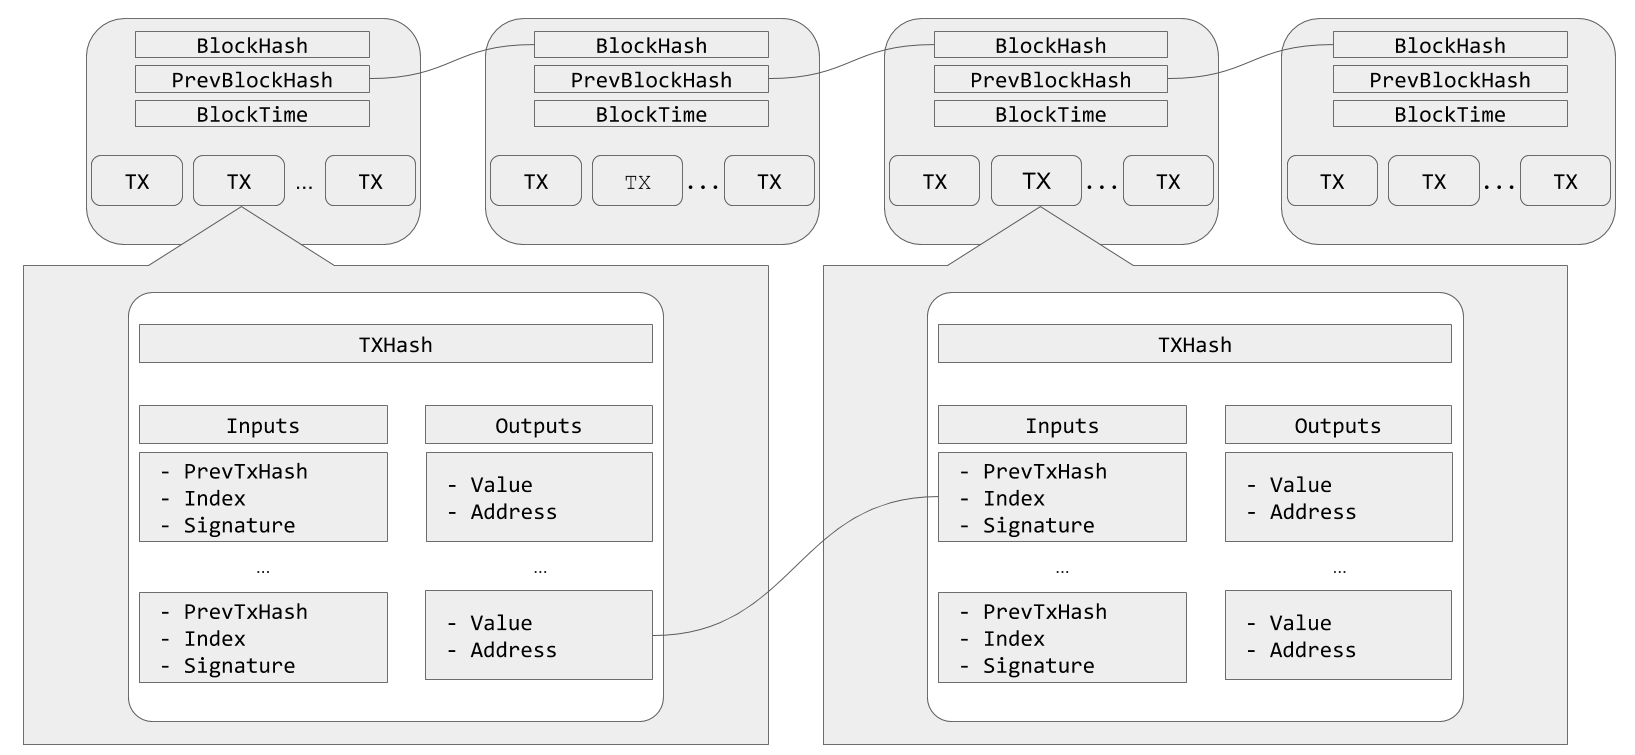
\includegraphics[width=0.8\linewidth]{fig/utxo_sys_HR}%
    \else%
    \fi%
  }%
  \caption{Blockchain and Transactions (adapted from \cite{tschorsch2016bitcoin}).}
  \label{fig:utxo_sys}
\end{figure*}

Recognizing the need for a more precise method, \cite{smith2017bitcoin} proposed
a cryptocurrency's \textit{turnover} as derivation of \ac{cdd}. %
We compare this approach to the other methods and show that, compared to
\ac{cdd}, the measure is indeed closer to the velocity estimates in many
tests. %




%%% Local Variables:
%%% mode: latex
%%% TeX-master: "../main"
%%% End:
% Related work
%Fischer and Stuff
\section{Theoretical concepts of measures for the velocity of money}
\label{sec:concepts}

% To facilitate an informed discussion of measures for the velocity of money,
% we first clarify the use of technical terms for the theoretical concepts. %

At its core, velocity of money refers to the average number of turnovers per
monetary unit within a period of time. %
This definition stems from the \emph{transaction form} of the quantity theory
of money as formalized by \cite{fisher1911equation}.%
\footnote{
  % The concept of relating money flows to monetary flows of goods and services has %
  % been put to writing first by \cite{humes1752ofmoney} but might have even older %
  % roots~\cite{volckart1997early}. %
  % Popularized by~\cite{fisher1911equation}, many different models arose. %
  % These are are summarized under the term \textit{quantity equations of money} today. %
  The transaction form highlights the use of money as a medium of exchange; %
  other forms stress different characteristics.  All forms, however, relate %
  money flows to real transactions. %
  While the transaction form is an identity and thus by definition correct, %
  it is nowadays mostly considered impractical for use in monetary %
  policy-making \citep[cf.][]{friedman2017quantity}. %
  General criticism was spurred by \cite{keynes2018general, tobin1989money, hansen1957american}, who reasoned that an unstable, %
  endogenously forming velocity of money would render the equations useless %
  for steering inflation. %
  The relation of monetary aggregates and price levels is disputed until this day \citep[cf.][]{dwyer1988money, mccallum2001monetary, gali2002new, bachmeier2005predicting, favara2009reconsidering}. 
  % As of definitional challenges to some of the theories %
  % central variables, the theory might better be formulated using income
  % transactions \cite{angell1936behavior} or focusing on the usefulness of
%   money as an asset rather than the mechanical payment process \cite{tobin1958liquidity}. %
}
%
The central equation of the theory equates the flows of real transactions,
given by the scalar product $\langle\Pp,\Tp\rangle$ of prices $\Pp$ and
transaction volumes $\Tp$, to total money flows, equal to the product of the
money supply $\Mp$ and its velocity \(\Vp\), where \(\perd\) denotes the time
period considered. %
With $n\in\mathbb{N}$ this amounts to
%
\begin{align}%
\label{eq:fisher}
  \Mp \Vp=\langle\Pp,\Tp\rangle\ \text{with}\ \Mp, \Vp \in \mathbb{R},\ 
  \text{and}\ \Pp,\Tp \in \mathbb{R}^{n}.%
\end{align}
The scalar product on the right-hand side is referred to as the \textit{price
  sum}.  In this product, \( \Pp=( \Pp_{1},\Pp_{2}, \cdots , \Pp_{n} ) \)
denotes a vector of prices $\Pp_t$ of transacted goods and services in
transaction $t$ during period $\perd$.  Transaction volumes \( \Tp \) are
given in units of goods and services. %
They are conceptualized as the vector %
\( \Tp=( \Tp_{1},\Tp_{2}, \cdots , \Tp_{n} ) \) %
with volume $\Tp_t$ in transaction $t$ in period $\perd$.  On the left-hand
side, $\Mp$ stands for the number of all units of money supply available in
period $\perd$. %
$\Vp$ denotes the velocity of money.%
\footnote{\label{sheep-note} To see this equation less abstractly, imagine an
  economy with only 2 gold coins, Alice, Bob and sheep Eve. %
  Alice owns the 2 gold coins and Bob the sheep Eve. %
  In $2020$, Alice buys Eve from Bob for 1 gold coin. %
  Later in the year, Bob regrets his decision and buys Eve back for the same
  price---Alice receives her coin back. %
  The quantity equation states the following:\\%
  %
  $ \displaystyle
  \begin{aligned}%
    2\,\coins \, \cdot \, V_{\mathtt{2020}} = %
    \langle\begin{pmatrix}%
    	1\,\frac{\coins}{\sheep} \\%
    	1\,\frac{\coins}{\sheep}%
    \end{pmatrix}, % 
    \begin{pmatrix}%
    	1\,\sheep \\%
    	1\,\sheep%
    \end{pmatrix}\rangle %
    = 2\,\coins.%
  \end{aligned} %
  $ \\%
  Now the velocity $V_{\mathtt{2020}}$ of the economy's money can be backed out
  as $1$.%
} %
%
While \(\Tp\), \(\Vp\) and \(\Pp\) are measured over a time period, \(\Mp\) %
is a point-in-time measure. %
To simplify, we assume the money supply is fixed during period \(\perd\)
and record it at the period's beginning \(\perd_\Start\). %

To develop intuition for velocity \(\Vp\), it can be viewed as weighted
average number of turnovers of all monetary units
\citep[cf.][]{friedman2017quantity}. %
The weights are derived from sorting the units into groups $g\in{}\Gp$ with
respect to their number of turnovers $\vp_g$ during period $\perd$. %
Velocity $\Vp$ then is%
\begin{align}\label{eq:velo_concept}%
  \Vp = \sum_{g\in\Gp}% 
  \Bigl(%
  \vp_g \cdot \frac{\Np_g}{\sum_{g\in\Gp} \Np_g}%
  \Bigr)%
  ,%
\end{align}%
with $\Np_g$ monetary units in group $g$ in period $\perd$. %
Velocity thus is the sum of turnover numbers~$\vp_g$, weighted by their
respective fractions.%
\footnote{%
  Returning to the example in footnote~\ref{sheep-note}, one coin was turned
  over twice---and one not at all. %
  Thus %
  $V_{\mathtt{2020}}= 0 \cdot \frac{%
    1\,\coins%
  }{%
    2\,\coins%
  } + 2\,\cdot \frac{%
    1\,\coins%
  }{%
    2\,\coins%
  }$. %
  This shows how the quantity equation is an identity and an implicit
  definition of velocity (rather than a testable statement, compare
  \cite{friedman2017quantity}).%
} %
While this definition is intuitive, it cannot be used to measure velocity in
practice. %
Turnover numbers per monetary unit are neither recorded for fiat currencies,
nor can they be inferred unambiguously for UTXO-based cryptocurrencies
% by counting transfers of coins
(compare \refsec{concept_utxo}). %
In practice, the velocity of money is thus backed out of \refequ{fisher}:
$V_\perd = \langle\Pp,\Tp\rangle/\Mp$. %

For cryptocurrencies, this appears a simple task, using on-chain transaction
volume and total coin supply. %
However, due to their technical implementation, transaction volumes recorded
on-chain are distorted. %
The next section therefore discusses the relevant subtleties of UTXO-based
cryptocurrency systems. %


%%% Local Variables:
%%% mode: latex
%%% TeX-master: "../main"
%%% End:
% Theoretic concepts of measures for the velocity of money
\section{UTXO-based cryptocurrencies}
\label{sec:concept_utxo}%

Bitcoin builds its transaction graph chaining transaction outputs. %
This approach is followed by many altcoins, referred to as %
\emph{UTXO-based cryptocurrencies}. %
UTXO refers to the ``coins'' that can be spent---\emph{unspent transaction
  outputs}.%
\footnote{For a detailed explanation of UTXO-based and account-based %
  cryptocurrency systems see \cite{zahnentferner2018chimeric}.} %
Thus, UTXO-based cryptocurrencies record only transactions, in contrast to
account-based cryptocurrencies which store a balance for each address on
their blockchain. %
% (compare \cite{zahnentferner2018chimeric})
As an extensive exposition is provided by \cite{tschorsch2016bitcoin}, we
restrict ourselves to features relevant for calculating velocity measures. %

UTXO-based cryptocurrency protocols ensure an ordered transaction history
using a linked chain of so-called \textit{blocks} (compare
\reffig{utxo_sys}). %
These blocks contain a hash ({\ttfamily\bfseries\slshape BlockHash})
fingerprinting the information of all transactions recorded in the block, a
timestamp ({\ttfamily\bfseries\slshape BlockTime}) and the hash of the
previous block ({\ttfamily\bfseries\slshape PrevBlockHash}). %
This constellation of hashes and timestamps establishes pointers that are
determining the order of blocks. %
The process of creating new blocks, called \emph{mining}, creates new
monetary units in so called \emph{coinbase transactions}. %
Creating blocks usually involves solving a computationally demanding puzzle
(\emph{proof-of-work}) or proving stake in the existing coin supply
(\emph{proof-of-stake}). %

Generally, transactions contain a hash as identifier
({\ttfamily\bfseries\slshape TxHash}) as well as inputs and outputs. %
Coinbase transactions are exceptions as they include an output but no
input. %
This effectively increases the amount of spendable outputs, and thus money in
the system. %
% Fees can be paid to miners by constructing a transaction with a lower sum
% of output than input values. %
Inputs are recorded as links back to outputs of a previous transaction
identified by an index ({\ttfamily\bfseries\slshape PrevTxHash}). %
Outputs can be sent to addresses ({\ttfamily\bfseries\slshape Address})
corresponding to public keys of an appropriately generated public--private
key pair. %
Unspent previous outputs can be used as inputs only upon proving ownership
({\ttfamily\bfseries\slshape Signature}). %
Generating this proof requires the private key belonging to the public key
which received the output. %
Importantly, transaction inputs can only be spent as a whole. %
If a fraction of the input is to be retained, an additional output must be
included which links to an address belonging to the spender. %
Such addresses are known as \textit{change addresses} and we refer to the
respective outputs as \textit{change outputs}. %

We refer to all outputs sent to an address controlled by the sender,
following~\cite{kalodner2017blocksci}, as \emph{self-churn}. %
Since the concept of \textit{user identities} does not exist in UTXO-based
cryptocurrencies, there is no direct way to clearly separate self-churn from
outputs transferred to third parties \citep[cf.][]{meiklejohn2013fistful}. %
Moreover, no relation between elements of the set of inputs and those in the
set of outputs of a transaction is determined. %
In other words, no technical link between individual outputs and inputs
exists; unspent outputs are fully fungible. %
Therefore, velocity measures cannot be calculated by following ``coins'' or
UTXOs through their transactions: due to splitting and rejoining within
blocks there exists no ``path'' the money took.

% Mixing services make use of the unspecified assignment between inputs and
% outputs of a transactions to obfuscate the link between transactions even
% further.%
% \footnote{%
% 	This practice is sometimes referred as \textit{coinjoins} where money from %
% 	different users is pooled in one transactions to shuffle the specific UTXOs %
% 	around. For a more detailed explanation refer to~\cite{moser2013inquiry}.%
% }%

%%% Local Variables:
%%% mode: latex
%%% TeX-master: "../main"
%%% End:
% UTXO based cryptocurrencies
%State-of-the-art estimations
\section{Self-churn and Clustering}
\label{sec:particularities_txvol}%
% 
As discussed in the last section, by construction many cryptocurrency
transactions contain outputs sending a fraction of the value back to the
sender. %
Such change outputs as well as other self-churn ought to be excluded from
transaction volume: %
%
\blockquote[%
\cite{fisher1922purch}%
]{%
  What is desired is the rate at which money is used for purchasing %
  goods, not for making change
}. %

\subsection{Transaction volume inflated by self-churn}
\label{sec:particularities_txvol:inflated}% 
While the transaction volume in principle can be calculated accumulating the
output values $\valO(o)$%
\footnote{To simplify notation, we denote many variables as functions of
  transactions, outputs or inputs. %
  For example, function $\valO(o)$ extracts the output value of output \(o\)
  of transaction \(t\) in period \(\perd\).} %
of all transactions $t$ recorded within period $\perd$ this yields an
inflated aggregate $\langle\Pp',\Tp'\rangle$ when defined as
\begin{align}%
  \langle\Pp',\Tp'\rangle = \sum_{t\in\TxP}\sum_{o\in\Out_\mathtt{t}} \valO(o),%
\end{align} %
with $o\in\Out_\perdT$ the set of all outputs of transaction $t$ in period
$\perd$ and \(\TxP\) the set of all transactions $t$ recorded within %
period $\perd$.  Thus, this volume needs to be adjusted. %
Defining $\Out^{\selfchurn}$ as the set of all self-churn outputs, the
accumulated transaction volume from these outputs $\Op$ can be obtained by
summing the individual self-churn outputs $c \in \Out^{\selfchurn}$ as%
\begin{align}%
  \Op = \sum_{t\in\TxP} \sum_{o\in\Out^{\selfchurn}} \valO(o).%
\end{align}%
Hence a corrected transaction volume can be calculated as %
$\langle\Pp,\Tp\rangle= \langle\Pp',\Tp'\rangle - \Op$.

Note that in practice we only observe the above transaction volume in terms
of monetary units rather than the full vector of prices and transacted
units. %
% These two are implicitly part of the measure $\langle\Pp,\Tp\rangle$.

\subsection{Adjustment heuristics to deflate transaction volumes}
\label{sec:particularities_txvol:adjustment_txvol}% 
%
As discussed in \refsec{concept_utxo}, only addresses but no identities are
recorded in the transaction ledger. %
This complicates the classifications of self-churn, needed to calculate
adjusted (deflated) transaction volume. %
However, statistical properties have been used to classify outputs as likely
belonging to the same individual user as the transactions inputs (compare
\cite{meiklejohn2013fistful}). %
While \emph{heuristics}, such procedures are now commonly employed to create
\emph{user clusters} of addresses. %
Outputs are classified as self-churn if the cluster of their destination
address equals the cluster of their input addresses. %

% Clustering addresses is has been done in various studies %
% (compare \cite{meiklejohn2013fistful}, \cite{spagnuolo2014bitiodine}, %
% \cite{herrera2014research} and many others). %

As our empirical analysis builds on a blockchain parser proposed
by~\cite{kalodner2017blocksci}, we follow their choice of heuristics. %
They employ one heuristic first proposed by~\cite{meiklejohn2013fistful} and
one accounting for \textit{peeling chains}. %
Peeling chains are transaction patterns where large unspent transaction
outputs are split into smaller amounts in a chain of transactions. %
Upon manual inspection \cite{kalodner2017blocksci} concluded that outputs
created and spent within a relatively short time period often belong to the
same user cluster. %
The heuristics used are thus:%
\begin{enumerate}\setlength{\itemsep}{0pt}
\item All inputs in a transaction stem presumably from one person.
  \footnote{%
    Note that \cite{kalodner2017blocksci} added the additional restriction
    that this heuristic is not applied to coinjoin transactions which are
    used to obfuscate transaction paths. %
    Coinjoin transaction are classified as in \cite{goldfeder2018cookie}.%
  } %
  % \item Addresses are only classified as change addresses if they are never reused as receipient. %
\item Outputs created and spent within 4 blocks are classified as self-churn
  transactions. %
\end{enumerate}%

%\subsection{Practical adjustment methods to deflate transaction volumes}\label{sec:particularities_txvol:adjustment_txvol}% 
%
% As our empirical analysis builds on a blockchain parser proposed %
% in~\cite{kalodner2017blocksci}, we simply adopt the default choice %
% % \footnote{\url{https://github.com/citp/BlockSci/wiki#toc-clustering-default-heuristic}} %
% of their package and form %
% clusters using the \emph{multi-input} heuristic proposed first %
% in~\cite{meiklejohn2013fistful} and an adjusted form of the \emph{optimal-change} heuristic introduced in
% \cite{nick2015data}. %
% %
% \par The multi-input heuristic assumes, that all inputs of a certain transaction can be assumed to belong to a certain user cluster. %
% While simple, the method enjoyed considerable coverage in research \citep{harrigan2016unreasonable, androulaki2013evaluating, herrera2014research} and is seen as effective measure of deanonymization \citep{frowis2019safeguarding, conti2018survey}. %
% However, the multi-input heuristic leads to unreasonable large clusters as of coinjoin transactions which are used to obfuscate transaction paths \citep{moser2017anonymous}. %
% \cite{kalodner2017blocksci} added additional restrictions %
% that this heuristic is not applied to coinjoin transactions. %
% Coinjoin transaction are classified as in \cite{goldfeder2018cookie}. %
% %
% \par The optimal-change heuristic assumes that if there is an output smaller than any of the inputs, this output can be classified as change \citep{nick2015data}. % 
% \cite{kalodner2017blocksci}, however, add the restriction that the output needs to be the first output sent to the respective address as Cryptocurrency Wallets generate fresh change addresses for change outputs. %

% As our emprical analysis builds on a blockchain parser proposed %
% in~\cite{kalodner2017blocksci}, we follow their approach to form %
% clusters using one heuristic that has been proposed first %
% in~\cite{meiklejohn2013fistful} and one heuristic accounting for %
% \textit{peeling chains}. %
% According to \cite{kalodner2017blocksci}, peeling chains are transaction %
% patterns that split large unspent transaction outputs into smaller amounts %
% in a chain of transactions. %
% Manual inspection lead \cite{kalodner2017blocksci} to the conclusion that outputs %
% that are created and spent during a relatively short time period are often %
% belonging to the same user cluster. %
% The heuristics used are thus:%
% \begin{enumerate}%
% 	\item All inputs used in a transaction are most likely from one %
%           person.%
%           \footnote{%
% 		As the basic idea leads to unreasonable large clusters, %
% 		\cite{kalodner2017blocksci} added additional restrictions %
% 		that this heuristic is not applied to coinjoin transactions %
%                 which are used to obfuscate transaction paths. %
%     	Coinjoin transaction are classified as in \cite{goldfeder2018cookie}.%
%     } %
% 	%\item Addresses are only classified as change addresses if they are never reused as receipient. %
% 	\item Outputs that are created and spent within 4 blocks, are classified as %
% 	self-churn transactions. %
% \end{enumerate}%
% Having formed user-clusters of addresses, outputs are classified as self-churn %
% if the cluster of their destination address equals the cluster of %
% their input addresses. %

\section{Velocity based on total money supply}
\label{sec:oldmeas}%
% Equipped with all necessary basics from both realms---economics and
% computer science---recently suggested methods of velocity measurement for
% cryptocurrencies are to be summarized. %
% Both approaches utilize the total coin supply as measure of the money supply
% $\Mp$ in equation \eqref{eq:fisher}. %
The quantity equation \eqref{eq:fisher} requires a measure of the money
supply $\Mp$. %
To our knowledge, all prior work has employed the sum total of ever-mined
coins as its measure. %
We denote this money-supply measure $\MTotalP$ and calculate it at the
beginning of each period $\perd$. %
\footnote{%
  As discussed in \refsec{concepts}, we simplify by assuming a fixed money
  supply over period $\perd$, using the amount at the beginning of the
  period. %
  Neither \cite{kalodner2017blocksci} nor \cite{athey2016bitcoin} clearly
  specify their adopted choice.} %
% %%% --- PLS ADD FORMULA:  (and delete "." prior to \footnote)
% as
% \begin{align}%
%   $\MTotalP$ = FORMULA.
% \end{align}
% %%% ---END PLS ADD formula.
In all common UTXO-based cryptocurrencies it is a deterministic function of
block height. %
Technically, $\MTotalP$ can be calculated as the aggregate of outputs from the set of coinbase transactions \( \TxC \) belonging to the set \( \mathbb{P} \) of all periods with a maximum block time smaller \(\perd_\Start\) and thus
\begin{align}%
  \MTotalP = \sum_{t \in \TxC} \valO(o).%
\end{align}%

Based on the quantity equation \eqref{eq:fisher}, the simplest measure of
velocity arises from dividing total transaction volume
$\langle \Pp'\Tp' \rangle$ by total coin supply $\MTotalP$, which was
described in~\cite{bolt2016value} and adopted by~\cite{ciaian2018price}. %
%
Formally,
\begin{align}%
  \VNaiveEstP = \frac{\langle\Pp',\Tp'\rangle}{\MTotalP}.%
\end{align}%
%
$\VNaiveEstP$ offers the advantages of providing a theoretically sound
interpretation and extremely simple calculation. %
Moreover, data for calculating $\VNaiveEstP$ (raw on-chain transaction volume
and total coin supply) are widely available. %
\footnote{Time-series data can be downloaded for free from %
  \url{www.blockchair.com}, \url{www.blockchain.com}, \url{www.btc.com}. %
  Also \url{www.blockwatch.cc} and many other data brokers provide the data.}
However, the result is biased: Self-churn transactions lead to an
overestimation of transaction volume. %
 
\cite{athey2016bitcoin} and \cite{kalodner2017blocksci} propose a similar
velocity measure. %
However, they clean the price sum from self-churn and get %
% For every period $\perd$ it is thus calculated as the ratio of price %
% sum~$\langle\Pp,\Tp\rangle$ divided by the complete money supply
% $\MTotalP$. %
%
% Velocity $\VTotalEst$ can thus be estimated as%
%
\begin{align}%
  \VTotalEst = \frac{\langle\Pp,\Tp\rangle}{\MTotalP}.%
\end{align}%
%
In line with \refsec{concepts}, both measures can interpreted as the turnover
of coins during period $\perd$ averaged over the total coin supply. %


%%% Local Variables:
%%% mode: latex
%%% TeX-master: "../main"
%%% End:
% State of the Art: Currently used estimation methodsmethods
%Contribution Section
\section{Velocity of money in effective circulation}
\label{sec:newmeas}%
%
While these measures advanced quantifying the velocity of cryptocurrencies,
they suffer from inaccuracy as money supply is defined as ``the aggregate of
all monetary units ever issued'' ($\MTotalP$).  We therefore propose a
measure based on the component of money that circulates effectively. %
Denoting this circulating amount $\MCircP$, our measure yields
\begin{align}%
  \label{eq:vcirc_concept}
  \VCircEstP = \frac{\langle\Pp,\Tp\rangle}{\MCircP}.%
\end{align}%
%
% $\VCircP$ handles re-activated money gracefully, allowing %
% for a deeper glance into the economics of the cryptocurrency markets. %
% If money supply responds to price trends, not only numerator but also %
% denominator change. %
% For more or less money in potentially being available for transactions, %
% $\VCircP$ reflects, whether this money indeed has been %
% used for processing transactions and to which degree. %

\subsection{Formal derivation}
\label{sec:formal-derivation}

To see how excluding hoarded money relates to the quantity theory, expand the
sum in \refequ{velo_concept} and differentiate the set of all monetary units
treated as investment, $h$, from its complement
$\GStrokeP\coloneqq\Gp\setminus\{h\}$:
\begin{alignat}{4}%
  \VTotalP%
  \ & = &\ & \vp_h \frac{%
    \Np_h%
  }{%
    \bigl( \Np_h+\sum_{g\in\GStrokeP} \Np_g \bigr)%
  }\\%
  \ & \ + &\ & \sum_{g\in\GStrokeP} \vp_g \frac{%
    \Np_g%
  }{%
    \bigl( \Np_h+\sum_{g\in\GStrokeP} \Np_g \bigr)%
  }.\nonumber%
\end{alignat}%
%
By definition, $h$ encompasses only non-transferred units, and thus $\vp_h=0$
in period $\perd$. Consequently %
% For a large fraction of money supply $\Np_z=0$ held %
% as investment, the respective turnover rate $\vp_z$ receives a %
% large weight %
% \begin{align}
% \frac{\Np_z}{\bigl( \Np_z+\sum_{g\in\GStrokeP} \Np_g \bigr)},
% \end{align} %
% while the components of actively used money supply receive a %
% small weight. %
% Velocity measured in the above way %
% thus yields values close to zero, making the variable slightly abstract in its %
% interpretation. %

% Money switching from \textit{hoarded} to \textit{in circulation} %
% increases or decreases the measure. %
% Thus, a change in the measure $\VTotalEstP$ could either mean that "effectively %
% circulating monetary units on average being turned over more times" or %
% "formerly illiquid monetary units are being now used for transactions". %
% %
% Measure $\VCircP$ reduces the equation to% 
\begin{align}%
  \label{eq:disentangle_vcirc}
  \VCircP %
  =  \sum_{g\in\GStrokeP} \vp_g
  \frac{\Np_g}{\sum_{g\in\GStrokeP} \Np_g },%
\end{align}%
% where group $h$, hoarded money, is not considered.
% , an interpretation of a change in $\VCircP$ can here clearly %
% be attributed to a higher intensity of turnover for the circulating money stock. %
% Assuming that self-churn transactions in the calculation of %
% the transaction volumes have been filtered out effectively, the measure %
% might be interpreted as a proxy for the %
% \textbf{average number of peer-to-peer hops that effectively circulating %
% 	money units where able to achieve} in period $\perd$. 
Hence, the measure can be interpreted as the average number of turnovers of
units effectively circulating in period $\perd$. %
Dropping non-circulating money in \refequ{disentangle_vcirc} amounts to an
adjustment of the money supply $\Mp$ in the quantity equation
\eqref{eq:fisher}.  %

\subsection{Theoretical basis and practical considerations}
An advantage of basing velocity on money in effective circulation is higher
information content. %
To begin with, it is questionable whether $\VNaiveEst$ and $\VTotalEst$
capture more information than transaction volumes $\langle\Pp,\Tp\rangle$,
respectively $\langle\Pp',\Tp'\rangle$. %
After all, for most UTXO-based cryptocurrencies money supply is just a simple
function of block height.%
\footnote{Difficulty adjustments for mining lead to close-to-constant spans
  between block creation times \citep{tschorsch2016bitcoin}.} %
% So far, there are only few cryptocurrencies that implement a responsive %
% money supply.%
% \footnote{%
%   Some so called ``stablecoins'' developed with the goal of a more stable %
%   purchasing power are trying to implement a coin supply matching the %
%   demand (compare \cite{klages2019stability}, \cite{routledge2018currency}, %
%   \cite{sidorenko2019stablecoin} \cite{pernice2019monetary} or \cite{bullmann2019search}).%
% } %
Thus, the two former measures appear very close to merely scaled versions of
their price-sums. %

Moreover, the total coin supply used in $\VNaiveEst$ and $\VTotalEst$
includes money that is technical dysfunctional (burnt coins). %
Yet also coins held unused as storage of wealth\footnote{Compare
  \cite{sawyer2003money} for a detailed discussion of the discrepancy arising
  from money as storage of wealth.} %
or speculation\footnote{Most studies conclude cryptocurrencies are currently used more for
  long-term speculation rather than as media of exchange %
  (see \eg \cite{%
    bouri2019herding,%
    anderson2019bitcoin,%
    yang2018behavioral,%
    yermack2015bitcoin%
  }).
  % The degree to which monetary units are hold unused can be %
  % seen e.g. in \cite{kalodner2017blocksci}, who find that over the last 10 years only roughly %
  % \SI{20}{\percent} of Bitcoins were %
  % spent again within a month. %
} %
do not fulfill one of the key functions of money, use as medium of exchange.%
\begin{figure*}[ht!]%
	\centering
	\ifdefined\varInputFigs%
%	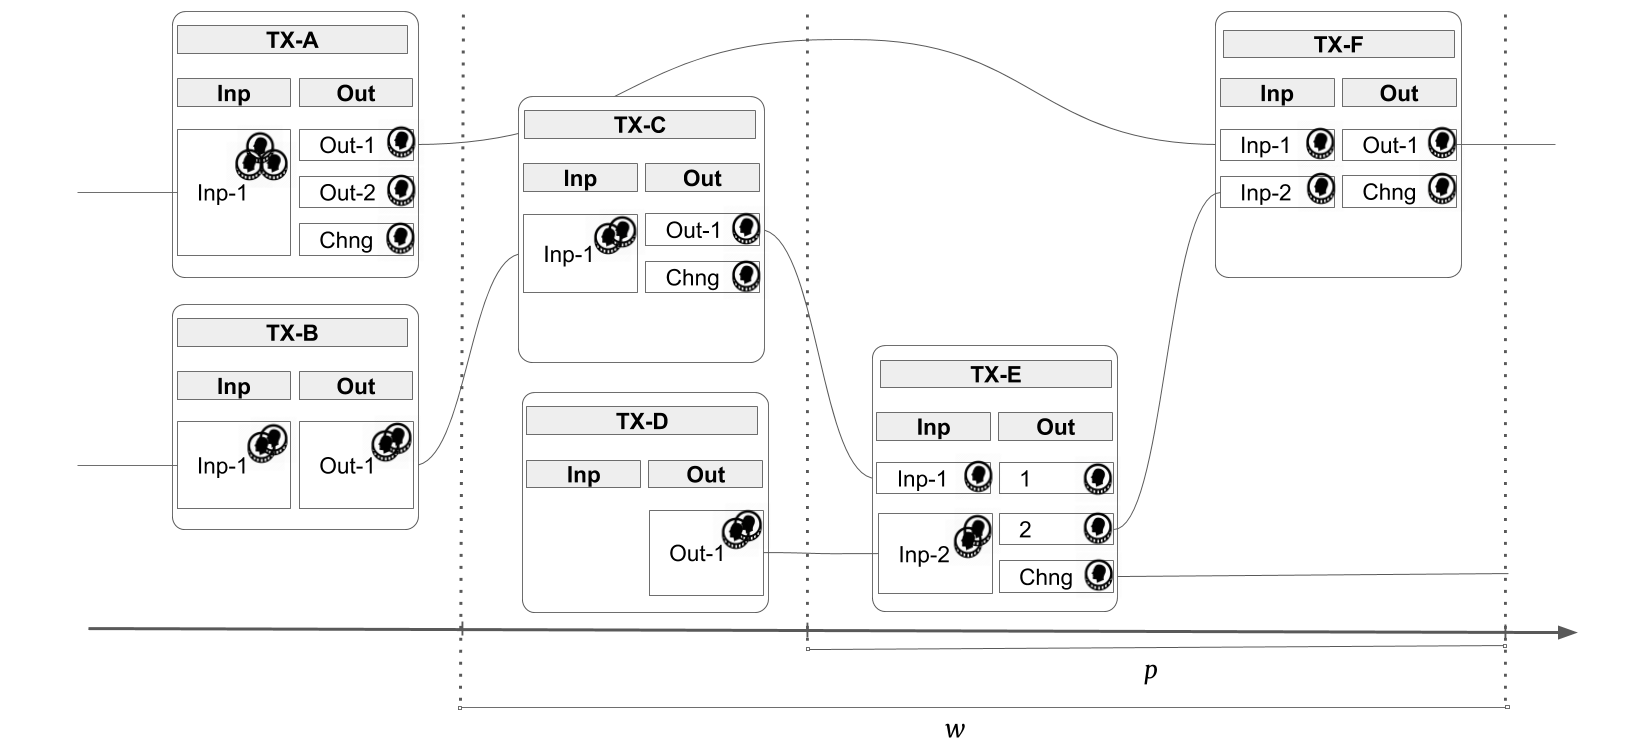
\includegraphics[width=0.8\linewidth]{fig/mcirc_concept_window_uneqal_period_HR}%
	%-------------------------------------------------------------------------------
\usetikzlibrary{calc}
%coordinate test point. Use as follows: 	\coordinate (cen) 	 	 at (0,0) (cen) [point];
\tikzset{
	every point/.style = {radius={\pgflinewidth}, opacity=1, draw, solid, fill=white},
	pt/.pic = {
		\begin{pgfonlayer}{foreground}
			\path[every point, #1] circle;
		\end{pgfonlayer}
	},
	point/.style={insert path={pic{pt={#1}}}}, point/.default={},
	point name/.style = {insert path={coordinate (#1)}}
}
%-------------------------------------------------------------------------------

% basic delacations
\pgfdeclarelayer{background}%
\pgfdeclarelayer{foreground}%
\pgfsetlayers{background,main,foreground}%

%Coin Symbol--------------------------------------------------------------------
\tikzset{%
	pics/coin/.style n args={3}{%
		code ={
			\def \coinLineWidth {#1}%
			\def \coinCenDist   {#2}%
			\def \circRad       {#3}%
			\def \signRad       {\circRad*0.20}%
			\def \signRadProp   {0.45}
			\def \signRadExt    {\signRad*\signRadProp}
			\def \signRadOut    {\signRad+\signRadExt}
			\def \signAngle     {30}
			\def \sinSignAngle  {sin(\signAngle)}
			\def \cosSignAngle  {cos(\signAngle)}
			\def \signWidth     {{pow((pow(\signRadOut,2)-pow(\sinSignAngle*\signRad,2)),0.5)-(\cosSignAngle)*\signRad)}}
			
			\def \startIX       {{cos(\signAngle)*\signRad}}
			\def \startIY       {{\sinSignAngle*\signRad}}
			
			\def \startOY       {\startIY}
			\def \signAngleOutS {{atan((\sinSignAngle*\signRad)/pow((pow(\signRadOut,2)-pow(\sinSignAngle*\signRad,2)),0.5))}}
			\def \signAngleOutE {{360-atan((\sinSignAngle*\signRad)/pow((pow(\signRadOut,2)-pow(\sinSignAngle*\signRad,2)),0.5))}}
	%
			\coordinate ()          at ( 0.0     , 0.0);%
			\coordinate (cen)       at ( 0.0     , 0.0);%
			\coordinate (cenB)      at ($(cen)    + ( 0.00,-\coinCenDist)$);%
						
			\node[
				circle,
				draw = black,
				fill = white,
				line width = \coinLineWidth,
				minimum size = \circRad,
				inner sep = 0pt,
				outer sep = 0pt,
			](NCD) at (cenB) {};
			
			\node[
				circle,
				draw = black,
				fill = white,
				line width = \coinLineWidth,
				minimum size = \circRad,
				inner sep = 0pt,
				outer sep = 0pt,
			](NCU) at (cen) {};
			
%			\draw[ - , line width = \coinLineWidth, black] (NCU.195) -- (NCD.195);
			\draw[-, line width = \coinLineWidth, black] (NCU.210) -- (NCD.210);
			\draw[-, line width = \coinLineWidth, black] (NCU.225) -- (NCD.225);
			\draw[-, line width = \coinLineWidth, black] (NCU.240) -- (NCD.240);
			\draw[-, line width = \coinLineWidth, black] (NCU.255) -- (NCD.255);
			\draw[-, line width = \coinLineWidth, black] (NCU.270) -- (NCD.270);
			\draw[-, line width = \coinLineWidth, black] (NCU.285) -- (NCD.285);
			\draw[-, line width = \coinLineWidth, black] (NCU.300) -- (NCD.300);
			\draw[-, line width = \coinLineWidth, black] (NCU.315) -- (NCD.315);
			\draw[-, line width = \coinLineWidth, black] (NCU.330) -- (NCD.330);
%			\draw[ - , line width = \coinLineWidth, black] (NCU.345) -- (NCD.345);
			
			\draw[
				 - ,
				 line width = \coinLineWidth,
				 black!80!white,
				 fill = black!80!white
			]
				(\startIX,-\startIY) arc (360-\signAngle:\signAngle:\signRad)
				-- +(\signWidth, 0.0)
				arc (\signAngleOutS:\signAngleOutE:\signRadOut)
				-- (\startIX,-\startIY)
				-- cycle
				;
		}%
		
	} ,%
	pics/coin/.default={1.0pt}{0.1}{1cm}%
}%
%
\begin{tikzpicture}
	\def \debugPoint   {}%
%b	\def \debugPoint   {point}%
	% font settings ############################################################
	\def \fontset      {\scriptsize\sffamily}
	% color definition #########################################################
	\def \colorOut     {black!100!white}
	\def \colorIn      {black!10!white}
	% arrow and line definitions ###############################################
	\def \lineW        {1.3pt}
	% width/height definition ##################################################
	\def \picW         {\linewidth*25.5/31}%
	\def \picH         {\paperheight*7.75/31}%
	\def \TH           {\picH*0.4}%picH*0.5*0.8
	
	\def \WBA          {\picW*11.50/31}
	\def \WLA          {\picW* 7.75/31}
	\def \WBB          {\picW* 4.00/31}
	\def \WLB          {\picW* 0.25/31}
	\def \WBC          {\picW* 3.50/31}
	\def \WBD          {\picW*10.50/31}
	\def \WLD          {\picW*14.25/31}
	% width/height nodes/boxes###################################################
	\def \BOH          {\picH* 0.35  }
	\def \BOW          {\picW* 6.0/31}
	
	% node positioning
	\def \BIPX         {\BOW*0.2375}
	
	% tikz styles################################################################
	\tikzstyle{lineIO} = [
		- ,
		line width = \lineW*0.8,
	]
	\tikzstyle{nodeOuter}   = [
		draw,
		rectangle,
		rounded corners=5pt,
		solid,
		line width = \lineW,
		black,
		inner sep = 0pt,
		outer sep = 0pt,
		text width = \BOW,
		minimum width = \BOW,
		minimum height = \BOH*1.075,
	]
	\tikzstyle{nodeInner}   = [
		draw,
		rectangle,
		rounded corners=3pt,
		solid,
		line width = \lineW*0.9,
		black,
		fill = \colorIn,
		inner sep = 0pt,
		outer sep = 0pt,
	]
	\tikzstyle{nodeInnerA}  = [
		nodeInner,
		align = center,
		text width = \BOW*0.9-3pt,
		minimum width = \BOW*0.9,
		minimum height = \BOH*0.15,
	]
	\tikzstyle{nodeInnerB}  = [
		nodeInner,
		align = left,
		text width = \BOW*0.425-5pt,
		minimum width = \BOW*0.425,
	]
	\tikzstyle{nodeInnerBA} = [
		nodeInnerB,
		minimum height = \BOH*0.15,
	]	
	\tikzstyle{nodeInnerBAC}b= [
		nodeInnerB,
		minimum height = \BOH*0.15,
		align = center,
	]
	\tikzstyle{nodeInnerBB} = [
		nodeInnerB,
		minimum height = \BOH*0.25,
	]
	\tikzstyle{nodeInnerBC} = [
		nodeInnerB,
		minimum height = \BOH*0.35,
	]
	\tikzstyle{nodeInnerBD} = [
		nodeInnerB,
		minimum height = \BOH*0.55,
	]
	% coordinates ###############################################################
	% 1 | 2 | 3 | 4 | 5 | 6 | 7 | 8 | 9 | 10 | 11 | 12 | 13 | 14 |
	% A | B | C | D | E | F | G | H | I |  J |  K |  L |  M |  N |
	
	\coordinate (cen)       at ($(0.0,0.0)   + ( 0.0       , 0.0         )$) (cen)   [\debugPoint];%
	
	\coordinate (PLU)       at ($(cen)       + (-\picW*0.5 , \picH*0.5   )$) (PLU)   [\debugPoint];%
	\coordinate (PLD)       at ($(cen)       + (-\picW*0.5 ,-\picH*0.5   )$) (PLD)   [\debugPoint];%
	\coordinate (PRU)       at ($(cen)       + ( \picW*0.5 , \picH*0.5   )$) (PRU)   [\debugPoint];%
	\coordinate (PRD)       at ($(cen)       + ( \picW*0.5 ,-\picH*0.5   )$) (PRD)   [\debugPoint];%
	
	
	\coordinate (TC)        at ($(cen)       + ( 0.0       ,-\TH         )$) (TC)    [\debugPoint];%
	\coordinate (TL)        at ($(TC)        + (-\picW*0.5 , 0.0         )$) (TL)    [\debugPoint];%
	\coordinate (TR)        at ($(TC)        + ( \picW*0.5 , 0.0         )$) (TR)    [\debugPoint];%
	
	\coordinate (BAC)       at ($(cen)       + (-\WBA      , 0.0         )$) (BAC)   [\debugPoint];%
	\coordinate (LAC)       at ($(cen)       + (-\WLA      , 0.0         )$) (LAC)   [\debugPoint];%
	\coordinate (BBC)       at ($(cen)       + (-\WBB      , 0.0         )$) (BBC)   [\debugPoint];%
	\coordinate (LBC)       at ($(cen)       + (-\WLB      , 0.0         )$) (LBC)   [\debugPoint];%
	\coordinate (LDC)       at ($(cen)       + ( \WLD      , 0.0         )$) (LDC)   [\debugPoint];%
	\coordinate (BCC)       at ($(cen)       + ( \WBC      , 0.0         )$) (BCC)   [\debugPoint];%
	\coordinate (BDC)       at ($(cen)       + ( \WBD      , 0.0         )$) (BDC)   [\debugPoint];%
	
	\coordinate (LAD)       at ($(LAC)       + ( 0.0       ,-\picH*0.5   )$) (LAD)   [\debugPoint];%
	\coordinate (LAU)       at ($(LAC)       + ( 0.0       , \picH*0.5   )$) (LAU)   [\debugPoint];%
	\coordinate (LBD)       at ($(LBC)       + ( 0.0       ,-\picH*0.5   )$) (LBD)   [\debugPoint];%
	\coordinate (LBDA)      at ($(LBC)       + ( 0.0       ,-\picH*0.4325)$) (LBDA)  [\debugPoint];%
	\coordinate (LBU)       at ($(LBC)       + ( 0.0       , \picH*0.5   )$) (LBU)   [\debugPoint];%
	\coordinate (LCD)       at ($(LDC)       + ( 0.0       ,-\picH*0.5   )$) (LCD)   [\debugPoint];%
	\coordinate (LCDA)      at ($(LDC)       + ( 0.0       ,-\picH*0.4325)$) (LCDA)  [\debugPoint];%
	\coordinate (LCU)       at ($(LDC)       + ( 0.0       , \picH*0.5   )$) (LCU)   [\debugPoint];%
	%coordinates, Box A Down, Tx_B		
	\coordinate (BADCC)     at ($(BAC)       + ( 0.0       ,-\picH*0.125 )$) (BADCC) [\debugPoint];%
	\coordinate (BADCL)     at ($(BADCC)     + (-\BIPX     , 0.0         )$) (BADCL) [\debugPoint];%
	\coordinate (BADCR)     at ($(BADCC)     + ( \BIPX     , 0.0         )$) (BADCR) [\debugPoint];%
	\coordinate (BADAC)     at ($(BADCC)     + ( 0.0       ,-\BOH *0.4   )$) (BADAC) [\debugPoint];%
	\coordinate (BADAL)     at ($(BADAC)     + (-\BIPX     , 0.0         )$) (BADAL) [\debugPoint];%
	\coordinate (BADAR)     at ($(BADAC)     + ( \BIPX     , 0.0         )$) (BADAR) [\debugPoint];%
	\coordinate (BADBC)     at ($(BADCC)     + ( 0.0       ,-\BOH *0.2   )$) (BADBC) [\debugPoint];%
	\coordinate (BADBL)     at ($(BADBC)     + (-\BIPX     , 0.0         )$) (BADBL) [\debugPoint];%
	\coordinate (BADBR)     at ($(BADBC)     + ( \BIPX     , 0.0         )$) (BADBR) [\debugPoint];%
	\coordinate (BADDC)     at ($(BADCC)     + ( 0.0       , \BOH *0.2   )$) (BADDC) [\debugPoint];%
	\coordinate (BADDL)     at ($(BADDC)     + (-\BIPX     , 0.0         )$) (BADDL) [\debugPoint];%
	\coordinate (BADDR)     at ($(BADDC)     + ( \BIPX     , 0.0         )$) (BADDR) [\debugPoint];%
	\coordinate (BADEC)     at ($(BADCC)     + ( 0.0       , \BOH *0.4   )$) (BADEC) [\debugPoint];%	
	%coordinates, Box A Up, Tx_A
	\coordinate (BAUCC)     at ($(BAC)       + ( 0.0       , \picH*0.3125)$) (BAUCC) [\debugPoint];%
	\coordinate (BAUCL)     at ($(BAUCC)     + (-\BIPX     , 0.0         )$) (BAUCL) [\debugPoint];%
	\coordinate (BAUCR)     at ($(BAUCC)     + ( \BIPX     , 0.0         )$) (BAUCR) [\debugPoint];%
	\coordinate (BAUAC)     at ($(BAUCC)     + ( 0.0       ,-\BOH *0.4   )$) (BAUAC) [\debugPoint];%
	\coordinate (BAUAL)     at ($(BAUAC)     + (-\BIPX     , 0.0         )$) (BAUAL) [\debugPoint];%
	\coordinate (BAUAR)     at ($(BAUAC)     + ( \BIPX     , 0.0         )$) (BAUAR) [\debugPoint];%
	\coordinate (BAUBC)     at ($(BAUCC)     + ( 0.0       ,-\BOH *0.2   )$) (BAUBC) [\debugPoint];%
	\coordinate (BAUBL)     at ($(BAUBC)     + (-\BIPX     , 0.0         )$) (BAUBL) [\debugPoint];%
	\coordinate (BAUBR)     at ($(BAUBC)     + ( \BIPX     , 0.0         )$) (BAUBR) [\debugPoint];%
	\coordinate (BAUDC)     at ($(BAUCC)     + ( 0.0       , \BOH *0.2   )$) (BAUDC) [\debugPoint];%
	\coordinate (BAUDL)     at ($(BAUDC)     + (-\BIPX     , 0.0         )$) (BAUDL) [\debugPoint];%
	\coordinate (BAUDR)     at ($(BAUDC)     + ( \BIPX     , 0.0         )$) (BAUDR) [\debugPoint];%
	\coordinate (BAUEC)     at ($(BAUCC)     + ( 0.0       , \BOH *0.4   )$) (BAUEC) [\debugPoint];%
	%coordinates, Box B Down, Tx_D	
	\coordinate (BBDCC)     at ($(BBC)       + ( 0.0       ,-\picH*0.1875)$) (BBDCC) [\debugPoint];%	
	\coordinate (BBDCL)     at ($(BBDCC)     + (-\BIPX     , 0.0         )$) (BBDCL) [\debugPoint];%
	\coordinate (BBDCR)     at ($(BBDCC)     + ( \BIPX     , 0.0         )$) (BBDCR) [\debugPoint];%
	\coordinate (BBDAC)     at ($(BBDCC)     + ( 0.0       ,-\BOH *0.4   )$) (BBDAC) [\debugPoint];%
	\coordinate (BBDAL)     at ($(BBDAC)     + (-\BIPX     , 0.0         )$) (BBDAL) [\debugPoint];%
	\coordinate (BBDAR)     at ($(BBDAC)     + ( \BIPX     , 0.0         )$) (BBDAR) [\debugPoint];%
	\coordinate (BBDBC)     at ($(BBDCC)     + ( 0.0       ,-\BOH *0.2   )$) (BBDBC) [\debugPoint];%
	\coordinate (BBDBL)     at ($(BBDBC)     + (-\BIPX     , 0.0         )$) (BBDBL) [\debugPoint];%
	\coordinate (BBDBR)     at ($(BBDBC)     + ( \BIPX     , 0.0         )$) (BBDBR) [\debugPoint];%
	\coordinate (BBDDC)     at ($(BBDCC)     + ( 0.0       , \BOH *0.2   )$) (BBDDC) [\debugPoint];%
	\coordinate (BBDDL)     at ($(BBDDC)     + (-\BIPX     , 0.0         )$) (BBDDL) [\debugPoint];%
	\coordinate (BBDDR)     at ($(BBDDC)     + ( \BIPX     , 0.0         )$) (BBDDR) [\debugPoint];%
	\coordinate (BBDEC)     at ($(BBDCC)     + ( 0.0       , \BOH *0.4   )$) (BBDEC) [\debugPoint];%
	%coordinates, Box B Up, Tx_C
	\coordinate (BBUCC)     at ($(BBC)       + ( 0.0       , \picH*0.2500)$) (BBUCC) [\debugPoint];%	
	\coordinate (BBUCL)     at ($(BBUCC)     + (-\BIPX     , 0.0         )$) (BBUCL) [\debugPoint];%
	\coordinate (BBUCR)     at ($(BBUCC)     + ( \BIPX     , 0.0         )$) (BBUCR) [\debugPoint];%
	\coordinate (BBUAC)     at ($(BBUCC)     + ( 0.0       ,-\BOH *0.4   )$) (BBUAC) [\debugPoint];%
	\coordinate (BBUAL)     at ($(BBUAC)     + (-\BIPX     , 0.0         )$) (BBUAL) [\debugPoint];%
	\coordinate (BBUAR)     at ($(BBUAC)     + ( \BIPX     , 0.0         )$) (BBUAR) [\debugPoint];%
	\coordinate (BBUBC)     at ($(BBUCC)     + ( 0.0       ,-\BOH *0.2   )$) (BBUBC) [\debugPoint];%
	\coordinate (BBUBL)     at ($(BBUBC)     + (-\BIPX     , 0.0         )$) (BBUBL) [\debugPoint];%
	\coordinate (BBUBR)     at ($(BBUBC)     + ( \BIPX     , 0.0         )$) (BBUBR) [\debugPoint];%
	\coordinate (BBUDC)     at ($(BBUCC)     + ( 0.0       , \BOH *0.2   )$) (BBUDC) [\debugPoint];%
	\coordinate (BBUDL)     at ($(BBUDC)     + (-\BIPX     , 0.0         )$) (BBUDL) [\debugPoint];%
	\coordinate (BBUDR)     at ($(BBUDC)     + ( \BIPX     , 0.0         )$) (BBUDR) [\debugPoint];%
	\coordinate (BBUEC)     at ($(BBUCC)     + ( 0.0       , \BOH *0.4   )$) (BBUEC) [\debugPoint];%
	%coordinates, Box C Down, Tx_E	
	\coordinate (BCDCC)     at ($(BCC)       + ( 0.0       ,-\picH*0.175 )$) (BCDCC) [\debugPoint];%	
	\coordinate (BCDCL)     at ($(BCDCC)     + (-\BIPX     , 0.0         )$) (BCDCL) [\debugPoint];%
	\coordinate (BCDCR)     at ($(BCDCC)     + ( \BIPX     , 0.0         )$) (BCDCR) [\debugPoint];%
	\coordinate (BCDAC)     at ($(BCDCC)     + ( 0.0       ,-\BOH *0.4   )$) (BCDAC) [\debugPoint];%
	\coordinate (BCDAL)     at ($(BCDAC)     + (-\BIPX     , 0.0         )$) (BCDAL) [\debugPoint];%
	\coordinate (BCDAR)     at ($(BCDAC)     + ( \BIPX     , 0.0         )$) (BCDAR) [\debugPoint];%
	\coordinate (BCDBC)     at ($(BCDCC)     + ( 0.0       ,-\BOH *0.2   )$) (BCDBC) [\debugPoint];%
	\coordinate (BCDBL)     at ($(BCDBC)     + (-\BIPX     , 0.0         )$) (BCDBL) [\debugPoint];%
	\coordinate (BCDBR)     at ($(BCDBC)     + ( \BIPX     , 0.0         )$) (BCDBR) [\debugPoint];%
	\coordinate (BCDDC)     at ($(BCDCC)     + ( 0.0       , \BOH *0.2   )$) (BCDDC) [\debugPoint];%
	\coordinate (BCDDL)     at ($(BCDDC)     + (-\BIPX     , 0.0         )$) (BCDDL) [\debugPoint];%
	\coordinate (BCDDR)     at ($(BCDDC)     + ( \BIPX     , 0.0         )$) (BCDDR) [\debugPoint];%
	\coordinate (BCDEC)     at ($(BCDCC)     + ( 0.0       , \BOH *0.4   )$) (BCDEC) [\debugPoint];%
	%coordinates, Box D Up, Tx_F
	\coordinate (BDUCC)     at ($(BDC)       + ( 0.0       , \picH*0.3125)$) (BDUCC) [\debugPoint];%	
	\coordinate (BDUCL)     at ($(BDUCC)     + (-\BIPX     , 0.0         )$) (BDUCL) [\debugPoint];%
	\coordinate (BDUCR)     at ($(BDUCC)     + ( \BIPX     , 0.0         )$) (BDUCR) [\debugPoint];%
	\coordinate (BDUAC)     at ($(BDUCC)     + ( 0.0       ,-\BOH *0.4   )$) (BDUAC) [\debugPoint];%
	\coordinate (BDUAL)     at ($(BDUAC)     + (-\BIPX     , 0.0         )$) (BDUAL) [\debugPoint];%
	\coordinate (BDUAR)     at ($(BDUAC)     + ( \BIPX     , 0.0         )$) (BDUAR) [\debugPoint];%
	\coordinate (BDUBC)     at ($(BDUCC)     + ( 0.0       ,-\BOH *0.2   )$) (BDUBC) [\debugPoint];%
	\coordinate (BDUBL)     at ($(BDUBC)     + (-\BIPX     , 0.0         )$) (BDUBL) [\debugPoint];%
	\coordinate (BDUBR)     at ($(BDUBC)     + ( \BIPX     , 0.0         )$) (BDUBR) [\debugPoint];%
	\coordinate (BDUDC)     at ($(BDUCC)     + ( 0.0       , \BOH *0.2   )$) (BDUDC) [\debugPoint];%
	\coordinate (BDUDL)     at ($(BDUDC)     + (-\BIPX     , 0.0         )$) (BDUDL) [\debugPoint];%
	\coordinate (BDUDR)     at ($(BDUDC)     + ( \BIPX     , 0.0         )$) (BDUDR) [\debugPoint];%
	\coordinate (BDUEC)     at ($(BDUCC)     + ( 0.0       , \BOH *0.4   )$) (BDUEC) [\debugPoint];%
	
	\coordinate (INPD)      at ($(cen)       + (-\picW*0.5 ,-\picH*0.195 )$) (INPD)  [\debugPoint];%
	\coordinate (INPU)      at ($(cen)       + (-\picW*0.5 , \picH*0.2425)$) (INPU)  [\debugPoint];%
	\coordinate (OUTU)      at ($(cen)       + ( \picW*0.5 , \picH*0.2950)$) (OUTU)  [\debugPoint];%
	
	%clipping
	\clip ($(PLD) + ( 0.0 ,-0.5)$) rectangle ($(PRU) + ( 0.0 , 0.1)$);
	%basic picture
	
	\draw[ ->, solid , line width = \lineW] (TL)   -- (TR);
	\draw[ - , dashed, line width = \lineW] (LAD)  -- (LAU);
	\draw[ - , dashed, line width = \lineW] (LBD)  -- (LBU);
	\draw[ - , dashed, line width = \lineW] (LCD)  -- (LCU);
	\draw[ - , gray  , line width = \lineW] (LBDA) -- node[midway, below, black]{$p$} (LCDA);
	\draw[ - , gray  , line width = \lineW] (LAD)  -- node[midway, below, black]{$w$} (LCD);
	%Nodes
	%node A Up, Tx_A
	\node[nodeOuter]   (NBAU)   at (BAUCC) {};	
	\node[nodeInnerA]  (NBAUEC) at (BAUEC) {\fontset{}$\mathsf{Tx_A}$};	
	\node[nodeInnerBAC](NBAUDL) at (BAUDL) {\fontset{}\textbf{Input}};	
	\node[nodeInnerBAC](NBAUDR) at (BAUDR) {\fontset{}\textbf{Output}};	
	\node[nodeInnerBD] (NBAUBL) at (BAUBL) {\fontset{}$\mathsf{Inp_1}$};	
	\node[nodeInnerBA] (NBAUCR) at (BAUCR) {\fontset{}$\mathsf{Out_1}$};
	\node[nodeInnerBA] (NBAUBR) at (BAUBR) {\fontset{}$\mathsf{Out_2}$};
	\node[nodeInnerBA] (NBAUAR) at (BAUAR) {\fontset{}Chng};
	
	%node A Down, Tx_B
	\node[nodeOuter]   (NBAD)   at (BADCC) {};	
	\node[nodeInnerA]  (NBADEC) at (BADEC) {\fontset{}$\mathsf{Tx_B}$};	
	\node[nodeInnerBAC](NBADDL) at (BADDL) {\fontset{}\textbf{Input}};	
	\node[nodeInnerBAC](NBADDR) at (BADDR) {\fontset{}\textbf{Output}};	
	\node[nodeInnerBD] (NBADBL) at (BADBL) {\fontset{}$\mathsf{Inp_1}$};	
	\node[nodeInnerBD] (NBADBR) at (BADBR) {\fontset{}$\mathsf{Out_1}$};
	
	%node B Up, Tx_C
	\node[nodeOuter]   (NBBU)   at (BBUCC)                      {};	
	\node[nodeInnerA]  (NBBUEC) at (BBUEC)                      {\fontset{}$\mathsf{Tx_C}$};	
	\node[nodeInnerBAC](NBBUDL) at (BBUDL)                      {\fontset{}\textbf{Input}};	
	\node[nodeInnerBAC](NBBUDR) at (BBUDR)                      {\fontset{}\textbf{Output}};	
	\node[nodeInnerBD] (NBBUBL) at (BBUBL)                      {\fontset{}$\mathsf{Inp_1}$};	
	\node[nodeInnerBC] (NBBUCR) at ($(BBUCR)+(0.0,-\BOH*0.10)$) {\fontset{}$\mathsf{Out_1}$};
	\node[nodeInnerBA] (NBBUAR) at (BBUAR)                      {\fontset{}Chng};
	
	%node B Down, Tx_D
	\node[nodeOuter]   (NBBD)   at (BBDCC) {};	
	\node[nodeInnerA]  (NBBDEC) at (BBDEC) {\fontset{}$\mathsf{Tx_D}$};	
	\node[nodeInnerBAC](NBBDDL) at (BBDDL) {\fontset{}\textbf{Input}};	
	\node[nodeInnerBAC](NBBDDR) at (BBDDR) {\fontset{}\textbf{Output}};	
	\node[nodeInnerBD] (NBBDBR) at (BBDBR) {\fontset{}$\mathsf{Out_1}$};
	
	%node C Down, Tx_E
	\node[nodeOuter]   (NBCD)   at (BCDCC)                     {};	
	\node[nodeInnerA]  (NBCDEC) at (BCDEC)                     {\fontset{}$\mathsf{Tx_E}$};	
	\node[nodeInnerBAC](NBCDDL) at (BCDDL)                     {\fontset{}\textbf{Input}};	
	\node[nodeInnerBAC](NBCDDR) at (BCDDR)                     {\fontset{}\textbf{Output}};	
	\node[nodeInnerBA] (NBCDCL) at (BCDCL)                     {\fontset{}$\mathsf{Inp_1}$};	
	\node[nodeInnerBC] (NBCDBL) at ($(BCDBL)+(0.0,-\BOH*0.1)$) {\fontset{}$\mathsf{Inp_2}$};	
	\node[nodeInnerBA] (NBCDCR) at (BCDCR)                     {\fontset{}$\mathsf{Out_1}$};
	\node[nodeInnerBA] (NBCDBR) at (BCDBR)                     {\fontset{}$\mathsf{Out_2}$};
	\node[nodeInnerBA] (NBCDAR) at (BCDAR)                     {\fontset{}Chng};
	
	%node D Up, Tx_F
	\node[nodeOuter]   (NBDU)   at (BDUCC)                      {};	
	\node[nodeInnerA]  (NBDUEC) at (BDUEC)                      {\fontset{}$\mathsf{Tx_F}$};	
	\node[nodeInnerBAC](NBUUDL) at (BDUDL)                      {\fontset{}\textbf{Input}};	
	\node[nodeInnerBAC](NBDUDR) at (BDUDR)                      {\fontset{}\textbf{Output}};	
	\node[nodeInnerBB] (NBDUCL) at ($(BDUCL)+(0.0,-\BOH*0.05)$) {\fontset{}$\mathsf{Inp_1}$};
	\node[nodeInnerBB] (NBDUCR) at ($(BDUCR)+(0.0,-\BOH*0.05)$) {\fontset{}$\mathsf{Out_1}$};
	\node[nodeInnerBB] (NBDUAL) at ($(BDUAL)+(0.0, \BOH*0.05)$) {\fontset{}$\mathsf{Inp_2}$};
	\node[nodeInnerBB] (NBDUAR) at ($(BDUAR)+(0.0, \BOH*0.05)$) {\fontset{}Chng};
	
	%Arrows depending on nodes
	\draw[lineIO] (INPD)        .. controls ($(INPD)        + ( 0.00, 0.00)$) and ($(NBADBL.west) + ( 0.00, 0.00)$) .. (NBADBL.west);
	\draw[lineIO] (INPU)        .. controls ($(INPU)        + ( 0.00, 0.00)$) and ($(NBAUBL.west) + ( 0.00, 0.00)$) .. (NBAUBL.west);
	\draw[lineIO] (NBADBR.east) .. controls ($(NBADBR.east) + ( 0.75, 0.00)$) and ($(NBBUBL.west) + (-0.75, 0.00)$) .. (NBBUBL.west);
	\draw[lineIO] (NBAUBR.0012) .. controls ($(NBAUBR.east) + ( 1.00, 3.95)$) and ($(NBDUCL.west) + ( 0.00,-0.45)$) .. (NBDUCL.west);
	\draw[lineIO] (NBBDBR.east) .. controls ($(NBBDBR.east) + ( 0.75, 0.00)$) and ($(NBCDBL.west) + (-0.75, 0.00)$) .. (NBCDBL.west);
	\draw[lineIO] (NBBUCR.east) .. controls ($(NBBUCR.east) + ( 0.75, 0.00)$) and ($(NBCDCL.west) + (-0.75, 0.00)$) .. (NBCDCL.west);
	\draw[lineIO] (NBCDBR.east) .. controls ($(NBCDBR.east) + ( 0.75, 0.00)$) and ($(NBDUAL.west) + (-0.75, 0.00)$) .. (NBDUAL.west);
	\draw[lineIO] (NBDUCR.east) .. controls ($(NBDUCR.east) + ( 0.00, 0.00)$) and ($(OUTU)        + ( 0.00, 0.00)$) .. (OUTU);
	
	%Coin Symbols
	\pic[] () at ($(NBAUBL.east) + (-\BOH*0.125,-\BOH*0.0375)$) {coin={0.7pt}{0.05}{\BOH*0.12}};
	\pic[] () at ($(NBAUBL.east) + (-\BOH*0.075, \BOH*0.0375)$) {coin={0.7pt}{0.05}{\BOH*0.12}};
	\pic[] () at ($(NBAUBL.east) + (-\BOH*0.115, \BOH*0.1100)$) {coin={0.7pt}{0.05}{\BOH*0.12}};
	\pic[] () at ($(NBAUAR.east) + (-\BOH*0.075, 0.0        )$) {coin={0.7pt}{0.05}{\BOH*0.12}};
	\pic[] () at ($(NBAUBR.east) + (-\BOH*0.075, 0.0        )$) {coin={0.7pt}{0.05}{\BOH*0.12}};
	\pic[] () at ($(NBAUCR.east) + (-\BOH*0.075, 0.0        )$) {coin={0.7pt}{0.05}{\BOH*0.12}};
	
	\pic[] () at ($(NBADBL.east) + (-\BOH*0.115,-\BOH*0.0375)$) {coin={0.7pt}{0.05}{\BOH*0.12}};
	\pic[] () at ($(NBADBL.east) + (-\BOH*0.075, \BOH*0.0375)$) {coin={0.7pt}{0.05}{\BOH*0.12}};
	\pic[] () at ($(NBADBR.east) + (-\BOH*0.115,-\BOH*0.0375)$) {coin={0.7pt}{0.05}{\BOH*0.12}};
	\pic[] () at ($(NBADBR.east) + (-\BOH*0.075, \BOH*0.0375)$) {coin={0.7pt}{0.05}{\BOH*0.12}};
	
	\pic[] () at ($(NBBUBL.east) + (-\BOH*0.115,-\BOH*0.0375)$) {coin={0.7pt}{0.05}{\BOH*0.12}};
	\pic[] () at ($(NBBUBL.east) + (-\BOH*0.075, \BOH*0.0375)$) {coin={0.7pt}{0.05}{\BOH*0.12}};
	\pic[] () at ($(NBBUCR.east) + (-\BOH*0.075, 0.0        )$) {coin={0.7pt}{0.05}{\BOH*0.12}};
	\pic[] () at ($(NBBUAR.east) + (-\BOH*0.075, 0.0        )$) {coin={0.7pt}{0.05}{\BOH*0.12}};
	
	\pic[] () at ($(NBBDBR.east) + (-\BOH*0.115,-\BOH*0.0375)$) {coin={0.7pt}{0.05}{\BOH*0.12}};
	\pic[] () at ($(NBBDBR.east) + (-\BOH*0.075, \BOH*0.0375)$) {coin={0.7pt}{0.05}{\BOH*0.12}};
	
	\pic[] () at ($(NBCDCL.east) + (-\BOH*0.075, 0.0        )$) {coin={0.7pt}{0.05}{\BOH*0.12}};
	\pic[] () at ($(NBCDBL.east) + (-\BOH*0.115,-\BOH*0.0375)$) {coin={0.7pt}{0.05}{\BOH*0.12}};
	\pic[] () at ($(NBCDBL.east) + (-\BOH*0.075, \BOH*0.0375)$) {coin={0.7pt}{0.05}{\BOH*0.12}};
	\pic[] () at ($(NBCDAR.east) + (-\BOH*0.075, 0.0        )$) {coin={0.7pt}{0.05}{\BOH*0.12}};
	\pic[] () at ($(NBCDBR.east) + (-\BOH*0.075, 0.0        )$) {coin={0.7pt}{0.05}{\BOH*0.12}};
	\pic[] () at ($(NBCDCR.east) + (-\BOH*0.075, 0.0        )$) {coin={0.7pt}{0.05}{\BOH*0.12}};
	
	\pic[] () at ($(NBDUAL.east) + (-\BOH*0.075, 0.0        )$) {coin={0.7pt}{0.05}{\BOH*0.12}};
	\pic[] () at ($(NBDUCL.east) + (-\BOH*0.075, 0.0        )$) {coin={0.7pt}{0.05}{\BOH*0.12}};
	\pic[] () at ($(NBDUAR.east) + (-\BOH*0.075, 0.0        )$) {coin={0.7pt}{0.05}{\BOH*0.12}};
	\pic[] () at ($(NBDUCR.east) + (-\BOH*0.075, 0.0        )$) {coin={0.7pt}{0.05}{\BOH*0.12}};		
\end{tikzpicture} 
	\else%
	\fi%
	\caption{%
		An example of a transaction chain. %
	}%
	\label{fig:mcirc_concept}%
\end{figure*}%

Furthermore, the amount of money frozen in speculative investments might not
be neutral to money flows or prices. %
Since the beginnings of monetary economics, currency speculation has been
associated with patterns in price levels. %
In \cite{fullarton1845regulation} and \cite{marx1872kapital}, the illiquid
component is considered a reservoir for neutralizing demand shocks and
excluded from the money supply. %
For \cite{keynes1930treatise} and \cite{commons2003institutional} hoarded
money, as destroyed money, is \emph{leakage} which must be compensated to
stabilise the price level. %
\cite{fisher1911equation} associates the rise in market prices for one of the
early fiat U.S.\ bank notes with a relation of speculation and circulating
money as well: ``speculation acted as a regulator of the quantity of
money.'' %

Our proposed measure captures precisely this velocity of money in effective
circulation.  %
This perspective is already present in current theoretical research on
cryptocurrency prices.  %
For instance, the model of \cite{bolt2016value} distinguishes demand for
transactions from demand for rational speculation.
%and assume that a fiat currency is serving as denominator of value. %
When using the quantity equation, they deduct coins bought and held as
speculative investment. % and adjust it to cope with exchange rates between
%cryptocurrency and fiat money. %
Their modified quantity equation relates the exchange rate between fiat and
cryptocurrency $S_{\perd}$ to the velocity of cryptocurrency in effective
circulation $\VCircP$ and the volume of transactions $\Tp^{\ast}$ denominated
in units of cryptocurrency as %
\begin{align}
  S_{\perd} = \frac{\Tp^{\ast} / \VCircP}{\MCircP}.
\end{align}

The speculators in the model purchase cryptocurrency units if traded prices
lie below their risk-adjusted, discounted expected future price.  %
With increasing aggregate speculative positions, the risk of marginal
speculative investments rises, lowering the price speculators are willing to
pay.  %
On the other hand, higher speculative positions imply reduced $\MCircP$ and
increase current price according to their modified quantity equation.  %
A similar relation between money in circulation and speculation is modelled in
\cite{athey2016bitcoin} as well.  %

Hence, implicitly or explicitly theoretical research already employs velocity
based on circulating money rather than the total money supply.  %
We close the gap in empirical research by operationalizing the
circulation-based velocity measure for UTXO-based cryptocurrencies.  %

% START: BRING BACK?
% \par Calculating velocity this way solves the bias by including %
% coins with lost private keys, as they are excluded as sub-component of money with a velocity of zero. %
% % Besides certain incomplete lists%
%b % \footnote{%
% % 	See for example \url{%
% % 		https://en.bitcoin.it/wiki/List_of_Major_Bitcoin_Heists,_Thefts,_and_Losses%
% % 	}%
% % }, %
% % there is currently no way to clearly disentangle to two. %
% While concrete numbers are hard to estimate, locking cryptocurrency forever by losing %
% the respective private keys is seen as a major challenge for %
% cryptocurrencies (compare \cite{meiklejohn2018top}). %
% END: BRING BACK?

% We therefore want to adopt a different approach, which might be summarized as "money is what money does."%
% \footnote{This phrase was coined by \cite{dalton1965primitive} as functional %
%   definition of money in response to a stream of academic arguments in %
%   search for a normative set of characteristics an asset should represent %
%   to be classified as "money".} %
% meaning that money which is not used for transactions but hoarded would be excluded. %
% In~\cite{fisher1911equation}, "money" is defined ambiguously as money in circulation. %
% "In circulation" might be just broadly referring to money hold by the %
% population with the potential to be used in transactions at any moment in %
% time---the approach used so far. %
% However, "in circulation" might also be referred to money that is, in deed, %
% moved within a certain period. %
% \footnote{This question frames a major debate in monetary policy research %
% which is the source the different money measures "MO", "M1", etc. that group %
% money components with similar liquidity.} %
% \par Given the hybrid role of cryptocurrencies, being designed as medium of exchange but %
% mostly used as speculative asset, segregation of the money supply is an %
% intuitive step.%
% Given the historic dominance of commodity money (e.g. coins and notes based on %
% precious metals), there are models trying to solve a similar challenge. %
% Based on \cite{fullarton1845regulation}, the so-called \textit{anti-quantity theory %
% of money} proposed by \cite{marx1872kapital} divides money supply into %
% \textit{money taking the form of hoards} and \textit{circulating} money. %
% % However, also \cite{fisher1911equation} noted that speculation might %
% % act as "[...] regulator of the quantity of money [...]". %
% For \cite{keynes1930treatise} and \cite{commons2003institutional} hoarded money, as %
% destroyed money, is ``[...] leakage [...]'' that needs to be compensated. %
% In \cite{fullarton1845regulation} and \cite{marx1872kapital} the illiquid %
% component is used as reservoir for demand shocks and excluded from %
% the quantity equation of money. %
% In- and outflow into the pool of circulating money is governed by the %
% \textit{law of reflux}. %
% Summarized, the law of reflux states that money leaves the pool of %
% hoards exclusively for enabling %
% trades---and flows back immediately after the trade has been accomplished. %
%
% \par Certain asset pricing approaches like~\cite{bolt2016value} or~\cite{athey2016bitcoin} %
% take up this thought and differentiate between money in circulation %
% and money hold as speculative investment. %
% Both model the price discovery processes to depend on the amount of money %
% effectively circulating. %
% This amount tightly interacts with money hoards from speculation leading to %
% feedback effects between speculation and price development via the supply of %
% money in circulation. %
% The degree to which monetary units are hold as long-term investments can be %
% seen e.g. in \cite{kalodner2017blocksci}, who find that over time only roughly %
% \SI{20}{\percent} of Bitcoins are %
% spent again within a month. %
% %
%

% Additionally, e.g., for Bitcoin it is yet unknown to the public whether the %
% money supply mined by Satoshi Nakamoto has just has stayed unused so far or %
% whether its keys have been destroyed. %
% \footnote{%
% 	According to an estimation by the cryptocurrency exchange \emph{BitMex} %
% 	over 600.000 Bitcoin might have been mined by %
% 	Satoshi Nakamoto---a pseudonym for the developer or developing group of %
% 	Bitcoin. Note that this is only a rough estimate based on the founders %
% 	mining behavior. %
% 	Compare \url{https://blog.bitmex.com/satoshis-1-million-bitcoin/}. %
% } %
%
% Depending on the application field of the velocity estimate, %
% this might be an advantage or disadvantage. %
% \footnote{In contrast, the large influence of monetary units switching from %
% $\Np_0$ to $\Np_11$ with $\vp_1 = 1$, might be desired when %
% using velocity as regressor in price predictions. %
% Then, however, one might argue that off-chain transactions on exchanges %
% should be taken into account as well, while they should be excluded when %
% utilizing the measure as estimate of "moneyness".} %
%
% Second, most cryptocurrencies are currently used mostly for speculation and %
% rarely for peer-to-peer transactions %
% (e.g. \cite{bouri2019herding}, \cite{corbet2019cryptocurrencies} or %
% \cite{yang2018behavioral}). %
% This, in turn, leads to a large fraction of unspent transaction outputs %
% being temporarily deprived from being used for transactions. %
% Appreciating cryptocurrency prices might draw large fractions of the %
% hoarding component into circulation, distorting measures for the %
% fundamental use of the cryptocurrency as medium of exchange.
% 
% More importantly, the radical exclusion of money supply unused for %
% processing transactions within a certain period leads to a very helpful interpretation:
% The velocity %
% $V_{\perd, name-for-new} = \frac{\Pp \Tp}{\MCircP}$ 
% of coins used within a certain period can be interpreted as %
% \textbf{the number of peer-to-peer hops}, the respective coins are %
% able to accomplish on average in that period.%
% The measure has a lower bound of 1, providing an intuitive means to compare %
% the use of different cryptocurrenes as medium of exchange. %
% \footnote{Note that the rather simplistic arithmetic formulation is made %
% concrete and applicable for UTXO-based cryptocurrencies in \refsec{oldmeas:sub:types}.} %
% This measure, in contrast to the Ricardian definition of the velocity of money, %
% is constructed to be robust against distortions from hype-driven single-hop %
% transactions to exchanges. %
% \todo{This is still somewhat weak. The more evidence here, the better we %
% can show why the world needs our measure.}
%
% While the Ricardian measure would increase with the surge of long-term %
% investments being transferred to exchanges and traded there off-chain, %
% the above measure only increases when the same coin performs various transactions. %
% We thus see the above measure as a useful indicator for the "moneyness" %
% of a cryptocurrency. %
% While cryptocurrency prices are a  simple and widely used success indicator, %
% a measure for the use of the digital asset for peer-to-peer transactions might %
% be a first step into the direction of a more fundamental valuation of cryptocurrencies. %
%
% % Separating the money stock into a hoarded, illiquid component and a liquid, %
% money-like component has, among others, been reviewed and criticized %
% by~\cite{likitkijsomboon2005marx} and \cite{roche1985marx}. %
% % The theory has been criticized from various perspectives. %
% While we apply certain aspects of the anti-quantity equation of money to %
% modify the classical velocity of money 
% with the goal of defining a well interpretable and robust measure for the %
% "moneyness" of a cryptocurrency , establishing the anti-quantity theory of %
% money as model of thought for cryptocurrencies is not the objective of %
% this paper. However, the application of the anti-quantity equation of money, %
% still can be seen as a deviation from mainstream economics that mandates %
% thorough justification.
% 
% Most importantly, it should be emphasized, that our velocity definition %
% draws only from three basic concepts within the anti-quantity theory of %
% money: %
% Firstly, the separation of the money stock into a investment-like and a %
% money-like component; secondly, the law-of-reflux described earlier and %
% lastly the tautological form of the of the money equation. %
% This mitigates several issues. %
% For example, an important point of criticism regarding the theory arises %
% around the argumentation chain around modeling the equality of the %
% price-sum of transactions and the product of the money supply and velocity. %
% The equality is established using supply-demand arguments \todo{Which ones?}, %
% which conflicts with the law-of-reflux establishing independence between %
% supply and value of money (\cite{likitkijsomboon2005marx}). %
% This indeed highlights a conceptional inconsistency of the anti-quantity %
% equation theory. %
% It still holds, however, that the equation establishes a tautology at %
% any given point in time when seen in isolation. %
% This tautology suffices as basis for a mechanical definition of the %
% velocity of money.
% 
% Also, cryptocurrency markets are very different from full-blown economies. %%
% One major point of criticism is that the law-of-reflux might draw an %
% improper picture of the economy. %
% Surges in the money-demand due to an increased demand for the transaction %
% volume of goods would be compensated entirely by money flowing from money %
% hoards into circulation. %
% Likewise, increases of the total money stock would be absorbed quickly %
% by the hoarding component of money (\cite{likitkijsomboon2005marx}). %
% While this indeed seems odd \todo{explain} for national economies, for %
% cryptocurrencies the situation is different: %
% It seems plausible, that an increase in the demand for transactions %
% (often for speculative reasons) %
% draws to a high degree from long-term invested money.%
% \footnote{%
%		And indication for that has been offered earlier in %
%		[missing diagram introduced already above].%
% } %
% Also it does not seem implausible at all, that newly mined coins are %
% flowing first into money hoards and are used in transactions only when needed. %
% 
% An indication might be offered by staleness of newly mined coins that is %
% illuminated in \textbf{[missing diagram [see above: 1.eD1, 1.eD2, 1.cD1 + 4.eD1]]}. %
%
% Many other points of criticisms refer to irreconcilability of the theory %
% with realities of national economies (compare \cite{lavoie1986marx}, %
% \cite{foley2005marx} or \cite{likitkijsomboon2005marx}) and fortunately %
% are of little importance to the application for cryptocurrencies. %
% \todo{If we feel fruity, we might make this an own section and argue for %
% that theory in more detail. I would favor a simple and quick justification though.}
% For example, it has been criticized that the theory impedes the explanation %
% of trade imbalances and shifts in the foreign exchange markets, leads to unrealistic %
% characterizations of the market for loans, and the assumption of banks %
% following the real bills doctrine (\cite{likitkijsomboon2005marx}). %
% 
% However, the theory might be criticized on a very fundamental level. %
% Hoarded money and money in circulation are lastly indistinguishable and %
% differ only in their velocity of money. Classical monetary theorists see %
% money hoards simply as a subgroup of money with a velocity of zero. %
% [Note: This is argument is just "mäh". ]
%

%%% Local Variables:
%%% mode: latex
%%% TeX-master: "../main"
%%% End:
% Our contribution: Velocity on a segregated money supply
%Segregation of money

\section{Novel measures of velocity of money in effective circulation}
\label{sec:cc_money_seg}%

Based on the concept of velocity of money in effective circulation as
clarified last section, we now propose algorithms to calculate velocity for
UTXO-based cryptocurrencies. %

\subsection{Determining money in circulation}
\label{sec:cc_money_seg:sub:mcirc_concept}% 

Conceptually, a monetary unit has circulated in a period if and only if it
has been used as a medium of exchange.  Therefore, first a time window must
be specified with respect to which monetary units are to be classified as
\emph{circulating} or not.  %
Money is referred to as circulating if it has been moved economically within
the last day, month, year or generally any time period $\wndw$ covering
$[\wndw_\Start , \wndw_\End]$. %

To identify the fraction of the money supply which circulated within $\wndw$,
we step trough every transaction recorded in period $\wndw$.  %
Transactions spending outputs generated before $\wndw$ as well as outputs
from coinbase transactions (seignorage) have the interpretation of bringing
an amount into circulation that corresponds to the value of spent outputs.  %
%%% NOTE: Why would fees be excluded here?? -> DISCUSS %%%hwe
All inputs referring to UTXOs generated \emph{within} period $\wndw$, on the
other hand, re-spend money which has already been counted as circulating.%
\footnote{To develop an intuition, remember the example of sheep Eve being
  sold and re-bought by Bob in $2020$.  %
  This time Bitcoin was used and Alice held unspent outputs of $2$ bitcoin
  from transactions $5$ years ago.  %
  The transaction formed by Alice to buy sheep Eve, $Tx_1$, spends her
  five-year-old output and generates a new one in 2020 which is controlled by
  Bob.  %
  When Bob buys Eve back, he pays with the output of $1$ bitcoin from $Tx_1$
  in a second transaction ($Tx_2$).  %
  For $\wndw = \perd = 2020$, the value of $Tx_1$ (1 bitcoin) originated
  prior to 2020 and is thus money brought into circulation.  %
  $Tx_2$, however, spent an output generated in 2020---an already counted
  monetary unit.  %
%In the example, thus $\MCirc_{2019}=1 \ttext{ Bitcoin}$. 
} %
% This can be illustrated with \reffig{mcirc_concept} where values are %
% symbolized with coins. %
% Here, we would need to determine, how many monetary units have made the %
% transaction volume $8$ (sum of outputs in C, D, E and F excluding
% self-churn) during period $\wndw$ possible. %
% In this example, we would need to focus on transactions A, B and D in
% contrast to transactions C and E which reused monetary unspent transaction
% outputs that have been generated within period $\wndw$. %

Note that we define the time window $\wndw$ within which spent coins are
considered as \emph{circulating} distinct from the period $\perd$ for which
the velocity measure is calculated, $ [\perd_\Start, \perd_{\End}]$.  This
distinction can be parametrized via a maximum length $\wndwLength$ of the
look-back window $\wndw$, where $\wndw_\Start = \perd_\Start - \wndwLength$
and $\wndw_\End = \perd_\End$.  %

The approach as characterized so far, however, does not account for two
technical properties of UTXO-based cryptocurrencies: %
First, transactions always spend prior transaction outputs in full.  %
Second, there exists no attribution of individual outputs to the inputs of a
transaction; thus it remains undefined which input corresponds to which
output(s).  %

The first property raises the question how to deal with transactions which
send back change: %
Should the sum of all inputs be considered \textit{in circulation,} as
technically all was transferred---or should only the fraction sent to third
parties be considered?  %
We analyze both choices, naming the first \ac{wba} and the second
\ac{mca}.  %
They are visualized in \reffig{mcirc_concept}.  %
The moved-coin approach considers only output $\mathsf{Out_1}$ of transaction
$\mathsf{Tx_C}$ as circulating, not the change output.  %
This approach captures the net economic value transferred to a third
party.  %
The \ac{wba} classifies the whole input of transaction $\mathsf{Tx_C}$ as
circulating.  %
This approach captures the amount of money that has been moved technically;
it can also be interpreted as revealed to be available for transactions.  %

In the \ac{mca}, the sum of inputs is counted as circulating only net of
change outputs.  %
However, due to the second property of UTXO blockchains ambiguous
constellations can occur: If for a given transaction one input was generated
within and one before $\wndw$, it remains unspecified which one corresponds
to the change output.  %

Transaction $\mathsf{Tx_F}$ in \reffig{mcirc_concept} illustrates the
point.  %
It has two inputs: $\mathsf{Inp_1}$ originated before period $\wndw$ and
$\mathsf{Inp_2}$ originated within $\wndw$.  %
If only amounts sent to third parties matter, it remains unclear which of the
two inputs funded the change output.  %
For $\mathsf{Inp_1}$, the transaction would not increase money in
circulation.  %
In contrast, if $\mathsf{Inp_2}$ funded the change output, the transaction
would increase the amount in circulation by $\mathsf{Inp_1}$. %

To resolve the ambiguity, an assignment rule between transaction inputs and
outputs is required.  %
% Utilizing the terminology of cost accounting,
We consider both endpoints on the spectrum of the age of the input assigned
to the change transaction and thus differentiate between \ac{lifo}, where
oldest inputs get assigned to outputs first, and \ac{fifo}, where it is the
other way around.  %

Naturally, with the \ac{wba} this differentiation is void.  %
Hence, we have three definitions of money in circulation, each a function of
the activity window length $\wndwLength$: %
Money in circulation for period $\wndw$ adopting the \ac{wba}
($ \MCircWbPWl $), and both the \ac{mca} with the \ac{lifo} rule
($ \MCircMlPWl $) and the \ac{fifo} rule ($ \MCircMfPWl $).

\subsection{Definition of velocity measures}
\label{sec:cc_money_seg:sub:}%

Based on the above definitions of money in circulation, three variations of
velocity can be calculated in accordance with \refequ{vcirc_concept}---one
per money aggregate.  %
%
All measures capture the average number of peer-to-peer coin turnovers of
effectively circulating monetary units in period $\perd$.  They concur in
capturing on-chain liquidity; they differ \wrt to definitions of
\textit{circulating monetary units} and assignment rules linking transaction
inputs to outputs.  %
% 
The first measure is based on $\MCircWbP$ and simply calculated as %
\begin{align}%
  \label{equ:VCircWbEstPWl}
  \VCircWbEstPWl = \frac{\langle\Pp,\Tp\rangle}{\MCircWbEstPWl}.%
\end{align}%
$\VCircWbP$ is recommended if a conservative measurement of coin turnover is
sought or additional assumptions about how to link inputs to outputs should
be avoided.
% 
The second and third measures are based on $\MCircMfPWl$ and $\MCircMlPWl$,
respectively:  %
\begin{align}%
  \label{equ:VCircMfEstPWl}
  \VCircMfEstPWl = \frac{\langle\Pp,\Tp\rangle}{\MCircMfEstPWl}, \\
  \VCircMlEstPWl = \frac{\langle\Pp,\Tp\rangle}{\MCircMlEstPWl}.%
  \label{equ:VCircMlEstPWl}
\end{align}%
%
$\VCircMfEstP$ and $\VCircMlEstP$ are more stringent on the definition of
money in circulation.  %
Their monetary aggregates do not count ``touched'' funds, but only amounts
transferred to somebody other than the sender.
% Another advantage of the two measures is lower boundedness at 1 if \(\perd\) is set equal to \(\wndw\) which allows for
% an intutive understanding of the circulation of coins.%
% \footnote{Every transaction, by construction, can draw at most its own
%   transaction value into circulation. %
%   Transaction volume in both, numerator and denominator, is calculated free of change money.} % 
However, this comes at the cost of the additional assumption with respect to the assignment rule between transaction inputs and outputs.  %

\subsection{Algorithmic implementation}
\label{sec:cc_money_seg:sub:mcirc_pract}%
Having defined three velocity measures, we now detail our technical approach
and the implementation.

Money in circulation under the \ac{wba} is measured as in
\refalgo{code_mcirc_wb}.  %
For every period $\wndw$, we loop over all transactions $t\in\TxW$ and add
their inputs to circulating money if they either reference outputs from
coinbase transactions, denoted by $\genByCoinbase(i)$, or outputs with
timestamps $\dateGen(i)$ before the first timestamp $\wndw_\Start$ of period
$\wndw$.  %
%
%  \footnote{In \reffig{mcirc_concept}, the algorithm would go trough %
%  transaction C (adding output $\mathsf{1}$ of transaction B, referenced by input $\mathsf{1}$ %
%  of transaction C), would then go to transaction D (finding no input at all), %
%  then to transaction E (skipping output $\mathsf{1}$ of transaction E but adding output $\mathsf{1}$ %
%  of transaction D as referenced by input $\mathsf{2}$ of transaction E) and so forth. %
% } %
%
%\ifdefined\varInputAlgos%
\renewcommand{\arraystretch}{1.5}%
\begin{algorithm*}[!h]%
	\DontPrintSemicolon
	\caption{Whole-bill-approach: Measurement of $\protect\MCircWb$ within period $\perd$ with look-back window $\wndw$.}\label{algo:code_mcirc_wb}%
	\KwData{$\wndw_\Start$                                    	    \tcc*{Beginn of look-back window $w$}}%
	\KwData{$\TxP$                                              	\tcc*{Set of transactions in period $\perd$}}%
%	\KwResult{$\MCircWb$                                           \tcc*{Money supply to be estimated within period $\perd$}}%
%
	$ \MCircWb \gets {0} $											\tcc*{Money supply to be estimated within period $\perd$}%
%
	\ForEach {$ t \in \TxP $                                      	\tcc*[]{Loop through transactions $t$ of period $\perd$}}%
	{%
		\ForEach {$ i \in \InpT $                                 	\tcc*[]{Loop through inputs $i$ of transaction $t$}}%
		{%
			\If{%
				$\dateGen(i)<\wndw_\Start$\ or\ $\genByCoinbase(i)$\label{algo:code_mcirc_wbCond}\tcc*{Was $i$ generated before $\wndw_\Start$/from a coinbase transaction?}%
			}{%
				$\MCircWb \gets{\MCircWb + \valI(i)}$				\tcc*{Update money supply}%
			}%
		}%
	}%
	return $\MCircWb$                                             	\tcc*{Result: Return estimated money in circulation within period $\perd$ for \ac*{wba}}%
\end{algorithm*}%
\else%
\fi%
%

Measuring money in circulation under the \ac{mca} is depicted in
\refalgo{code_mcirc_mc}.  %
%
As in \refalgo{code_mcirc_wb}, for time window $\wndw$ we loop over all
transactions $t\in\TxP$ and add inputs based on the same core condition
(compare lines~\ref{algo:code_mcirc_mc}-\ref{algo:code_mcirc_mcCond} and
\ref{algo:code_mcirc_wb}-\ref{algo:code_mcirc_wbCond}).  %
This time, however, inputs are added step by step---only until the amount
sent to third parties is reached.  %
The order of inputs to consider is determined by the \ac{lifo} or \ac{fifo}
principle.  %
For every transaction $t$ in time window $\wndw$, the amount sent to third
parties is determined net of self-churn as
$\valO^\sendToOthers(t) = \sum_{o\in{}\Out'_{t}} \valO(o)$ %
where $\Out'_{t}$ denotes non-self-churn outputs of transaction $t$.  %
If all outputs are identified as self-churn, $\valO^\sendToOthers(t) = 0$ and
the algorithm continues with the next transaction.  %
%
If $\valO^\sendToOthers(t) > 0$, the algorithm collects input values in a
vector $\InpSortedT$; they are sorted in either ascending (\ac{lifo}) or
descending (\ac{fifo}) order \wrt to the timestamp when the UTXOs were
generated.  %
Then, looping over inputs $i$, input values $\valI(i)$ are added to
$\MCircMPWl(t)$ if they meet the core condition (compare line 17) introduced
in line 6 of \refalgo{code_mcirc_wb}.  %
\footnote{Summands $\MCircMPWl(t)$ can be interpreted as money drawn into
  effective circulation by transaction $t$.} %
However, one additional condition applies: If the last added input would
increase the summand $\MCircMPWl(t)$ beyond the value of outputs sent to
third parties $\valO^\sendToOthers(t)$, we only add up to the latter
amount.  %
% This effectively adds only the necessary fraction of the inputs of
% transaction $t$, generated before window $w$ or from coinbase transactions,
% that were required to match $\valO^\sendToOthers(t)$.  %

  % The components $\MCircMPWl(t)$ are consecutively summing all transaction
  % values to calculate money in circulation $\MCircMPWl$ for the given period
  % $p$ with respect to time window $\wndw$ as well as the applied sorting type.

% \par While our algorithms theoretically might be applied to any window length $\wndwLength$, in practice they lack performance for large windows. %
% Additional methods of optimization might be needed, to apply the method windows larger then 30 days. %


\subsection{Manipulation potential}
\label{sec:cc_money_seg:manipul}% 

One important concern with any measure of economic activity asks, how
amenable is it to manipulation?  In the case of velocity, the question is
specifically if the measure can be inflated by a single agent (or a small
group) of limited means.  After all, one proxy variable for velocity has been
designed as a manipulation-proof alternative to turnover (see
\refsec{results:sub:approx_crypto:subsub:bdd}).  How easy would it be to
create fake velocity in order to inflate our measures?

Indeed, no direct technical impossibility prevents generating transactions
affecting Equations~(\ref{equ:VCircWbEstPWl})--(\ref{equ:VCircMlEstPWl}).
Nonetheless, there exist reasonably tight limits to the manipulation
potential of our measures, in particular compared to trading volumes on
exchanges.

First and foremost, calculating our measure on on-chain transactions puts an upper
limit to fake transfers.  First, a fake transaction needs to be committed to
the blockchain, and thus can be repeated only once per block time.  As long
as the manipulator is not the miner confirming the next block (a random and
unlikely outcome even for large pools), the on-chain settlement is also
costly, incurring fees.

Second, the manipulator must fully fund her fake transactions: she cannot
send more than she owns once per block.  The question then turns to how she
should structure the fake transfers.  Send the entire amount in a single
transaction, or split it up into as many as can fit into a block?  In the
latter case, the fees rise.  In the former, should she minimize or maximize
the number of outputs?  If she maximizes, the fees rise again, and she
quickly fragments her wealth across a diverging multitude of wallets,
reducing the funds available in each for the next round (block) of
manipulation.

In this context it is critical that we follow the literature in clustering
user addresses: As long as the clustering works, the manipulator cannot
combine her funds ever again, lest she would be deconspired as a single agent
and all her fake transactions disregarded.  It follows that her strategy
minimizes the number of outputs, generating a chain of fresh addresses across
which a large sum, tied up in the manipulation, traverses indefinitely to
make-believe ``newcomers.''  This, however, matches peeling transactions,
which we also exclude.  She would thus need to break frequently enough in
order to escape this classification, slowing her manipulation further.

% More importantly, this strategy appears highly specific to game a measure
% which we only introduce in this paper.  Moreover, it is also straightforward
% to detect and exclude in the future.

% In sum, we are unaware of why anyone should want to pay to inflate our
% measures (unlike exchange turnover), who has the cryptocurrency funds and
% willingness and expertise to conduct such a technically elaborate
% manipulation.

In sum, manipulation attempts are both technically elaborate and relatively
straightforward to detect and exclude in the future. %
We thus do not consider manipulation a serious concern for our current
results, nor for our measures.

% 
%%% Local Variables:
%%% mode: latex
%%% TeX-master: "../main"
%%% End:
%% Segregating the money supply for UTXO-based cryptocurrencies

%%%Local Variables:
%%% mode: latex
%%% TeX-master: "../main"
%%% End:
% Velocity measu fanficres based on circulating money
%State of the Art Proxies
%
%%% Local Variables:
%%% mode: latex
%%% TeX-master: "../main"
%%% End:
% State of the Art: Currently used proxy methods
% Results

\section{Benchmarking popular velocity proxies on the Bitcoin blockchain }
\label{sec:results}%

Equipped with our proposed velocity measures that are calculated on a level
of detail of each output in each transaction in each block on the blockchain,
we can now use these measures to empirically assess the quality of popular
proxies for velocity.

To this end, we first review the most common proxies in
\refsec{results:sub:approx_crypto}, then implement the proposed estimators to
calculate velocity measures for Bitcoin in \refsec{results:sub:comp}, and
finally run tests in \refsec{results:sub:goodness} to evaluate the goodness
of fit of the proxies \wrt the measures.

\ifdefined\varInputAlgos%
\renewcommand{\arraystretch}{1.5}%
\begin{algorithm*}[!h]%
	\DontPrintSemicolon
	\caption{Whole-bill-approach: Measurement of $\protect\MCircWb$ within period $\perd$ with look-back window $\wndw$.}\label{algo:code_mcirc_wb}%
	\KwData{$\wndw_\Start$                                    	    \tcc*{Beginn of look-back window $w$}}%
	\KwData{$\TxP$                                              	\tcc*{Set of transactions in period $\perd$}}%
%	\KwResult{$\MCircWb$                                           \tcc*{Money supply to be estimated within period $\perd$}}%
%
	$ \MCircWb \gets {0} $											\tcc*{Money supply to be estimated within period $\perd$}%
%
	\ForEach {$ t \in \TxP $                                      	\tcc*[]{Loop through transactions $t$ of period $\perd$}}%
	{%
		\ForEach {$ i \in \InpT $                                 	\tcc*[]{Loop through inputs $i$ of transaction $t$}}%
		{%
			\If{%
				$\dateGen(i)<\wndw_\Start$\ or\ $\genByCoinbase(i)$\label{algo:code_mcirc_wbCond}\tcc*{Was $i$ generated before $\wndw_\Start$/from a coinbase transaction?}%
			}{%
				$\MCircWb \gets{\MCircWb + \valI(i)}$				\tcc*{Update money supply}%
			}%
		}%
	}%
	return $\MCircWb$                                             	\tcc*{Result: Return estimated money in circulation within period $\perd$ for \ac*{wba}}%
\end{algorithm*}%
\else%
\fi%
%%
%
% line numbering
%
\renewcommand{\LinesNumbered}{%
	\setboolean{algocf@linesnumbered}{true}%
	\renewcommand{\algocf@linesnumbered}{\everypar={\nl}}}%

\let\oldnl\nl% Store \nl in \oldnl
\newcommand{\nonl}{\renewcommand{\nl}{\let\nl\oldnl}}% Remove line number for one line

\ifdefined\varInputAlgos%
\renewcommand{\arraystretch}{1.90}%
%\todo{Do we mean non-recycling or not circulating?}%
\begin{algorithm*}[!h]%
	\DontPrintSemicolon
  \caption{Moved-coin-approach: Measurement $\protect\MCircM$ for $\mathtt{type}$ (\acs*{fifo}, \acs*{lifo}) within period $\perd$, window $\wndw$.%
  }\label{algo:code_mcirc_mc}%
%
	\KwData{$\wndw_\Start$ \tcc*{Beginn of look-back window $w$}}%
	\KwData{$ \TxP$                                                                     \tcc*{Set of transactions in period $\perd$}}%
	\KwData{$ \Out^{\selfchurn}$                                                        \tcc*{Set of self-churning outputs}}%
%	\KwResult{$\MCircM$                                                                 \tcc*{Money supply to be estimated in period $\perd$ with window $\wndw$}}%
%
	$\MCircM \gets {0}$																	\tcc*{Money supply to be estimated in period $\perd$ with window $\wndw$}%
%
	\ForEach {$ t \in \TxP $%
%		                                                            \tcc*{Loop through each transaction $t$ in period $\perd$}%
	                                                            }%
	{%
		$\MCircM(t) \gets {0}$                                                          \tcc*{Set summand of $\MCircM(t)$ for every transaction $t$}%
		$\valO^\mathtt{break}(t) \gets {0}$                                             \tcc*{Set break condition helper for every transaction $t$}%
		$\Out'_{t} \gets{\Out_{t}\setminus{}O^{\selfchurn}}$                            \tcc*{Determine the set of outputs of $t$ excluding self-churning outputs}%
		$\valO^\sendToOthers(t)  \gets{\sum_{o\in{}\Out'_{t}} \valO(o)}$                \tcc*{Amount of money sent to third parties}%
		\If{$\valO^\sendToOthers(t) = 0$}{%
			continue                                                                    \tcc*{Skip current transaction and go to the next}%
		}%
	    $\InpSortedT(\mathtt{type}) \gets{\InpT\ \text{sorted ascending (\acs*{fifo})/descending (\acs*{lifo}) according to $\mathtt{type}$ and thus generation time of inputs}}$\\%
	    \nonl\mbox{}\tcc*{$\InpT$ is the unsorted set of all inputs of $t$}%
	    \ForEach {$i \in \InpSortedT(\mathtt{type})$     \label{algo:code_mcirc_mc_for}%
%	    	                                              \tcc*{Loop through each input $i$ of sorted input set $\InpSortedT$}%
    	}{%
	    	$\valO^\mathtt{break} \gets{\valO^\mathtt{break} + \valI(i)}$\\%
			\If {
				$\dateGen(i)<\wndw_\Start$\ or\ $\genByCoinbase(i)$\label{algo:code_mcirc_mcCond}\tcc*{Was $i$ generated before $\wndw_\Start$/from a coinbase transaction?}
			}{%        
				$ \MCircM(t) \gets{\MCircM(t) + \valI(i)} $									\tcc*{Update money supply}%	
				\If{%
					$\valO^{\mathtt{break}}(t) > \valO^\sendToOthers(t)$ 					\tcc*{Update foreach-loop break helper}%
				}{%
					\If{%
						$\MCircM(t) > \valO^\sendToOthers(t)$								\tcc*{Use $\valO^\sendToOthers(t)$ as upper cap for  $\MCircM(t)$}%
					}{%
						$\MCircM(t) \gets{ \valO^\sendToOthers(t) }$%      		       
					}{%
						break                                                               \tcc*{Break foreach-loop on line \ref{algo:code_mcirc_mc_for} and proceed with line \ref{algo:code_mcirc_mc_break}}%
					}% 
				}%       
			}%   
		}%
	   	$ \MCircM \gets{\MCircM + \MCircM(t)} $\label{algo:code_mcirc_mc_break}%
	}%
	return $\MCircM$                                                                    \tcc*{Result: Return estimated money in circulation in period $\perd$ with window $\wndw$ for \ac*{mca}}%
\end{algorithm*}%
\else%
\fi%
%
\vspace*{1em}%
\renewcommand{\captionGlo} {Descriptives for velocity proxies and measures
  with $\perd = \wndwLength = 1 \ttext{ day}$ for 2013-06-01 to 2019-06-01.}%
\renewcommand{\labelGlo}{\label{tbl:descriptives_est_and_app}}%
\tableTwoColumnH{descriptives_est_and_app}%
% We assume that the availability of public price data marks the beginning of
% bitcoins being used as media of exchange.
% \footnote{While the results for \ac{mae}, \ac{mse} and \ac{msc} tests hold in equivalently also for data from 2009 onwards, the Minzer-Zarnowitz regressions does not allow for conclusive interferences.}%

\subsection{Popular proxy variables for velocity of UTXO-based
  cryptocurrencies}
\label{sec:results:sub:approx_crypto}%
% The following approximations are commonly used so far.

% \subsubsection{Turnover}
% \label{sec:results:sub:approx_crypto:subsub:turn}%
% Classical \emph{turnover} refers to the simple sum total of transacted
% amounts within a period $\perd$:%
% \begin{align}
%   \TurnoverP = \sum_{t\in\TxP} \sum_{i\in\InpT} \valI(i).%
% \end{align}

% Of course, modified variants of turnover can be constructed based on
% excluding change transactions, or transactions within user clusters.

% The main advantage is its simplicity and immediate correspondence to turnover
% as understood in classical financial markets.  It lacks the scaling by the
% money supply central to the concept of velocity, but it can still be used as
% a proxy for velocity measures based on total supply---which for
% cryptocurrencies after all is locally close to flat for short periods, and
% importantly, is (in contrast to fiat currencies) exogenously determined.

\subsubsection{Coin Days Destroyed}
\label{sec:results:sub:approx_crypto:subsub:bdd}%

Since turnover can be gamed via repeated transfers of an agent to
herself,\footnote{Primarily, allegations centered on exchanges inflating
  trading volumes to pretend to be more liquid.} %
the \Ac{cdd} measure was introduced as a manipulation-proof alternative in
\url{bitcointalk.org} in 2011.%
\footnote{\url{https://bitcointalk.org/index.php?topic=6172.msg90789\#msg90789}} %
For each input, \emph{coin days} refer to the product of its monetary value
and the number of days ``since it was last spent,'' \ie how many days the
funding output had remained a UTXO.  %
\Ac{cdd} then is defined as the sum of coin days over all transactions within
a period $\perd$:%
\begin{align}%
  \BddP = \sum_{t\in\TxP} \bdd(t),%
\end{align}%
where%
\begin{align}%
  \bdd(t) = \sum_{i\in\InpT}  \Delta(i) \cdot \valI(i)%
\end{align} %
with $\Delta(i)$ denoting the number of days since the respective input
originated as output (or coinbase transaction) in a prior block, and
$ \valI(i)$ the value of input $i$ of transaction $t$ in period $\perd$.  %
% For transactions $t=1$ to $\Tp$ for period $\perd$, this can be %
% calculated using the volume of transaction $t$ including fees %
% $\val^{\tx^{+}}_\perdT$ %
% and the weighted average days $\Delta \tp_t$ since the transaction $t$ of period $\perd$ has last been spent:%
% \begin{align}\label{eq:bdd}%
%   \BddP = \sum_{t=1}^{\Tp} \Delta \tp_t \cdot \val^{\tx^{+}}_\perdT,%
% \end{align}%
% where %
% \begin{align}%
%   \val^{\tx^{+}}_\perdT %
%   = \sum_{o=1}^{O_\perdT} \val^{\out}_{\perdTi} %
%   + \val^{\mathtt{fees}}_\perdT %
%   = \sum_{i=1}^{\Ip_t} \valI(\perdTi).%
% \end{align}%
% \Ac{cdd} was initially introduced by \emph{ByteCoin} as resilient %
% measure of transaction volume, unbiased by sending money back and forth artificially. %
% However, user \emph{MoonShadow} quickly brought it into discussion as measure %
% for the velocity of money. %$

The \Ac{cdd} measure puts larger weight on the reactivation of long-dormant
coins compared to ones frequently spun, a feature clearly differing from the
concept of velocity. %

\subsubsection{Turnover based on dormancy}
\label{sec:results:sub:approx_crypto:subsub:dorm}%

In \cite{smith2017bitcoin} a proxy for velocity, aiming at ``the average number of times the actively used
[coins] can be expected to turn over'' was proposed. %
While named ``turnover'' in \cite{smith2017bitcoin}, this is not to be confused with the classical \emph{turnover} that refers to the simple sum total of transacted
amounts within a period $\perd$:%
\begin{align}
  \TurnoverP = \sum_{t\in\TxP} \sum_{i\in\InpT} \valI(i).%
\end{align}
The measure in \cite{smith2017bitcoin} in contrast is constructed as the
inverse of average dormancy $\DormP$ multiplied by the time period, where
dormancy amounts to \ac{cdd} scaled by the sum of inputs spent during the
period $\perd$ \citep[cf.][]{smith2017bitcoin}:%%
% % BEGIN SHORTENING?
% \cite{smith2017bitcoin} developed dormancy as a measure for the average time that %
% coins have been hold unused before being transacted. %
% It is calculated as the weighted average days $\Delta \tp_t$ passed since %
% the last transaction. %
% As weights, the respective transaction volumes $\val^{\tx^{+}}_{t}$ relative to %
% the aggregated transaction volumes over period $\perd$ are used:
% \begin{align}%
%   \DormP %
%   = \frac{%
%   		\sum_{t\in\TxP}\Delta \tp_t \val^{\tx^{+}}_{t}%
%   	}{%
%   		\sum_{t\in\TxP} \val^{\tx^{+}}_{t}%
%   	} .%
% \end{align}%
% The number of weighted average days $\Delta \tp_t$ since the transaction has %
% last been spend %
% can be calculated%
% \footnote{
%   In the published working paper of \cite{smith2017bitcoin} it remains %
%   unclear, how the author conceptualizes this variable exactly. %
%   We thus suggest an appropriate definition of $\Delta \tp_t$.
% } %
% from the values of transaction inputs %
% $\valI(\perdTi)$ and the days since the spent input %
% has been generated in a preceding transaction $\Delta t_{\perdTi} $ as%
% \begin{align}%
%   \Delta \tp_t %
%   = \frac{%
%   	\sum_{i\in\InpPT}\Delta t_{\perdTi} \valI(\perdTi)%
%   }{%
%   	\sum_{i\in\InpPT} \valI(\perdTi)%
%   }.%
% \end{align}%
% %
% % END SHORTENING?
\begin{align}%
  \TurnP = \frac{1}{\DormP} \cdot  \delta,%
\end{align}%
with%
\begin{align}%
  \DormP = \frac{\BddP}{\sum_{t\in\TxP} \sum_{i\in\InpT} \valI(i)}.%
\end{align}%
Here $\delta$ refers to the length of the period for which turnover is
calculated.  %
To illustrate the concept, assume the coins spent today stayed unused on
average for 6 hours before their transaction.  %
Hence, circulating coins are turned over
$\frac{\SI{24}{\hour}}{\SI{6}{\hour}} = 4$ times per day on average.  %
Dormancy-based turnover, however, remains an approximation depending on
transactions distributed homogeneously over time.  %
% To see that, consider an example where there is only one coin %
% that is spend $5$ times rapidly over and over again in the first minutes %
% of the day. After that, nothing happens. The inferred approximation could be arbitrarily high depending on how little time passes %
% between the transactions. %
\renewcommand{\labelGlo}    {\label{fig:globfigComponents}}%
\renewcommand{\captionLocL} {Components of velocity measures.}%
\renewcommand{\captionLocR} {Correlations between the measures and price.}%
\renewcommand{\labelLocL}   {\label{fig:subfigComponentsPlot}}%
\renewcommand{\labelLocR}   {\label{fig:subfigComponentsCorr}}%
\figureTwoColumn{ts_figs/desc_components}{ts_figs/corrplot_components}%
\renewcommand{\captionGlo}  {Time series plots for proxy-variables.}%
\renewcommand{\labelGlo}    {\label{fig:globfigApp}}%
\renewcommand{\captionLocL} {Normalized variables of volatility approximation.}%
\renewcommand{\captionLocR} {Standardized variables of volatility approximation.}%
\renewcommand{\labelLocL}   {\label{fig:subfigAppNorm}}%
\renewcommand{\labelLocR}   {\label{fig:subfigAppStand}}%
\figureTwoColumn{ts_figs/desc_all_app_norm}{ts_figs/desc_all_app_stand}%

\subsection{Data sources and calculations}%Origin and description of approximation and measurement data}
\label{sec:results:sub:comp}%

%%% First data:
We collect a dataset spanning from June 2013 until June 2019, starting with
the rise of the first cryptocurrency exchanges and thus reliable trading
data. %

For the proxy variables, we tap existing sources as far as possible.  %
\Ac{cdd} data is gathered via API from
Blockwatch,\footnote{\url{https://blockwatch.cc}} %
trading data taken from
CoinMarketCap.\footnote{\url{https://coinmarketcap.com}}  %

To calculate the velocity measures, however, access to the atomic units of
cryptocurrency transactions is needed.  %
We rely on the open-source blockchain parser \emph{BlockSci} introduced by
\cite{kalodner2017blocksci}.  %
We also provide the code of our paper at
\url{https://github.com/wiberlin/ccurr_velocity/}. %
In replicating the clustering approach of \cite{kalodner2017blocksci} (see
\refsec{particularities_txvol:adjustment_txvol}), in order to mitigate the
amount and effect of false positives we exclude one unreasonably large
cluster with over 297 million addresses.  %
\footnote{Only 13 clusters contain more than $20,000$ addresses.}  %

%%% Then calculations:
We calculate our velocity measures based on a time window for money in active
circulation $\wndwLength$ equal to period $\perd = 1 \text{ day}$.%
\footnote{We define days based on transaction block times and UTC
  timezone.} %
Therefore, a \textit{coin} is in circulation if it is transferred at least
once within the day for which velocity is computed.  %
This daily measure can be interpreted as average turnover of monetary units
which are part of the daily circulating money supply.  %
While our choice for the window $\wndwLength$ within which moved coins are
considered actively in circulation is short, this allows us to flesh out the
difference between velocity based on the total money supply and our proposed
measures based on circulating supply most clearly.  Moreover, since
\cite{kalodner2017blocksci} provide results with an
implicitly\footnote{\cite{kalodner2017blocksci} equate money in circulation
  with total coin supply, implying an infinite time window.}  %
infinite $\wndwLength$, we provide evidence on the opposite endpoint on the
spectrum.  %
Naturally, neither the BlockSci parser nor our approach are restricted to
these choices and can be extended both to other time windows and other
UTXO-based cryptocurrencies.  %
% Calculating a daily velocity, for example, it might be interesting to base %
% the measure on money that circulated within the last week, month or year. %
% Analyzing the impact of the time window selection on velocity and its %
% relationship to returns or volatility might be highly interesting but %
% is left for future research. %
% In this section, we will display central characteristics of %
% approximation and estimator data and compare them from different perspectives. %

%%% Then properties of the calculated numbers:
\reftbl{descriptives_est_and_app} shows descriptive statistics for the
proxies and the measures.  %
$\Bdd$ denotes \ac{cdd} in million coin days, while $\Turn$ denotes
\emph{active turnover} in expected on-chain coin transfers.  %
For both proxy variables, means exceed medians, suggesting outliers in the
skewed distribution.  %
% 
According to $\VNaiveEst$, a monetary unit of the total coin supply is turned
over $0.11$ times on average, while the more sophisticated measure
$\VTotalEst$ results in turnover of $0.09$.  %
The difference stems from the deflated transaction volume used by
$\VTotalEst$ being strictly lower then the inflated one (see
\refsec{particularities_txvol}).  %
According to the measure $\VCircWbEst$, which is based on the \ac{wba}, coins
in effective circulation during the day reach turnover of around $5.83$.  %
Assuming the clustering heuristics work well, coin transfers correspond to
peer-to-peer hops.  %
Accordingly, $\VCircWbEst$ estimates that monetary units in circulation
change owners $5.83$ times per day, while $\VCircMfEst$ and $\VCircMlEst$ give
an estimate of around $6.09$ peer-to-peer hops.  %
The reason for the higher turnover estimate is the more conservative
operationalization of the concept of \textit{being in circulation} (see
\refsec{cc_money_seg:sub:mcirc_pract}).  %

The different levels can be disentangled by looking at the components of the
velocity measures.  %
\reffig{subfigComponentsPlot} exemplarily shows this for the components of
$\VTotalEst$ and $\VCircWbEst$.  %
While $\MTotal$ increases steadily over time, the subset of coins transacted
at least once per day, with an average \SI{1.5}{\percent} of the total
supply, is minuscule but volatile in comparison.%
\footnote{Compare appendix \ref{tbl:appendix_desc_other},
  \ref{tbl:appendix_desc_other_norm}, \ref{tbl:appendix_desc_other_stand} and
  \ref{tbl:corrtable_all} for additional descriptive statistics on the
  dataset.}  %
The deflated on-chain transaction volume varies widely---clearly always below
total supply, yet above the supply in circulation.  %
While the volatility in the transaction volume feeds fully into $\VTotalEst$,
for $\VCircWbEst$ the relation is less obvious.  %
In \reffig{subfigComponentsCorr}, the components' co-variation with bitcoin
price indicates that not only deflated on-chain transaction volume
$\mathtt{Vol}$, but also the monetary aggregates are positively correlated
with price changes.  %
% While this provides only anecdotal evidence, it is consistent with the
% hypothesis that transaction volumes as well as the liquid component of the
% money supply rise with price, and in consequence lower the correlation of the
% velocity measure $\VCircWbEst$ with price.  %
% This hypothesis is related to the broader question how far speculation might
% act as ``regulator of the quantity of money'' \citep{fisher1911equation}.  %
Somewhat surprising the velocity measures show a slightly negative correlation
with prices however. %
% 
\renewcommand{\captionGlo}{Components of velocity measures
  $\protect\VTotalEst$ and $\protect\VCircWbEst$ with
  $\perd = \wndwLength = 1 \ttext{ day} $.}%

Comparing maxima and minima across time series, as
\reftbl{descriptives_est_and_app} shows, requires scaling.  %
We use two methods: normalization and standardization.  %
Normalization is based on the usual %
$X^{norm} = (X-X_{min})/(X_{max}-X_{min})\in[0, 1]$.  %
Standardization is based on Z-scores
$X^{stand} = \frac{X-\mu(X)}{\sigma(X)},$ with mean $\mu(\cdot)$ and standard
deviation $\sigma(\cdot)$.  Both are sensitive to outliers
\citep[cf.][]{angelov2019empirical}, so we truncate at $10$ standard
deviations around the mean.%
\footnote{This procedure truncated a maximum of 3 values across time
  series.}  %
%
\reffig{globfigApp} shows the time series of proxy variables for velocity.  %
The scaling leads to a visible difference, relevant when comparing proxies to
measurement results.  %
A first indication of the quality of the proxy variables is their
diversity.  %
Not only spikes but also general trends vary across methods.  %
%
\reffig{globfigEst} depicts the different velocity measures.  %
Differences across measures are smaller, highs and lows correspond more. %
% The figure further shows the similarity between \ac{wba} and \ac{mca}. %
The next section provides quantitative evidence.

\renewcommand{\captionGlo}   {Time series plots for volatility measures with $\perd = \wndwLength = 1 \ttext{ day} $.}%
\renewcommand{\labelGlo}     {\label{fig:globfigEst}}%
\renewcommand{\captionLocL}  {Normalized variables of volatility measurement.}%
\renewcommand{\captionLocR}  {Standardized variables of volatility approximation.}%
\renewcommand{\labelLocL}    {\label{fig:subfigEstNorm}}%
\renewcommand{\labelLocR}    {\label{fig:subfigEstStand}}%
\figureTwoColumn{ts_figs/desc_all_est_norm}{ts_figs/desc_all_est_stand}%

\subsection{Assessing the goodness of fit of the proxies}
\label{sec:results:sub:goodness}%
We now turn to evaluate the proxy variables for velocity based on our
estimated measures.  %
In so doing, we include the trivial velocity measure $\VNaiveEst$ in the set
of proxies, as it is calculated on very high-level inputs (raw on-chain
transaction volume and total coin supply) that are similarly easy to obtain
as \ac{cdd} or \emph{turnover}.%
% \footnote{Note that \ac{cdd} for Bitcoin are available at 
%   many free blockchain explorers. \emph{Turnover} can, in combination with the 
%   daily inflated transaction volume, be inferred from the latter.} 

In order to evaluate the quality of proxy variables perfectly, the ``true''
velocity ought to be known.  At the same time, we have proposed three novel
measures, in addition to those suggested by \cite{athey2016bitcoin} and
\cite{kalodner2017blocksci}.  We do not view this a contradiction: after all,
the measures capture different concepts of velocity.  Ours, for example,
address the velocity of money in circulation.  Therefore, we do not horserace
all proxies against one benchmark, but rather evaluate the goodness of fit of
the proxy variables with any of the measures.  We do, however, take the
position that the measures are more precise estimators of ``true velocity''
(its respective concepts) than the proxies, and thus evaluate the latter
in terms of their fit to the former.

Perhaps surprisingly, the results do not vary qualitatively much across
different measurement approaches. %, so our results do not depend on a certain
%velocity measure.  %

\subsubsection{Approximation errors}
\label{sec:results:sub:comp:subsub:errors}%
A common approach assesses approximation errors by comparing \aclp{mse} or
\aclp{mae}.  %
\ac{mse}, by squaring them, punishes large deviations more rigorously than
the linear \ac{mae}.  We provide both, not only to the standardized and
normalized time series, but also on their first differences.  %
This is motivated, as in econometric studies like those in \refsec{lit}, by
doubts about the stationarity of the time series.  %

\reftbl{errortable} shows that the above transformations differ in their
assessment of the goodness of fit of approximation methods.  %
When judging by the normalized but undifferenced dataset, \emph{turnover}
$\Turn$ (as alternatively defined by \cite{smith2017bitcoin}) achieves the
lowest error in approximating velocity measures based on effectively
circulating money supply.  %
However, for all other constellations we find that the trivial measure
$\VNaiveEst$ provides the closest fit to all ways to measure velocity.  %


\subsubsection{Model confidence set test}
\label{sec:results:sub:comp:subsub:mcs}%
To understand if the approximation methods indeed differ significantly, we
perform \acf{mcs} tests.  %
\cite{hansen2011model} introduced \Ac{mcs} tests to measure the performance
of forecasting methods, but they are applicable more generally.  %
The method uses equivalence tests and an elimination procedure to determine
which set of models significantly outperforms the rest of the models.  %
For an intuitive understanding of the test one might think of a set $M$ of
models (here the different approximation methods).  %
The models are indexed using $i \text{ and } j \in 1,..,m $.  %
When comparing model $i$ to a benchmark, for each period $\perd$ model $i$
leads to loss functions
$ L_{i \perd} = L(V^{\est}_\perd, V^{\app}_{i \perd})$, where
$V^{\est}_\perd$ denotes the benchmark velocity measure and
$V^{\app}_{i \perd}$ the approximation method $i$.

To compare the performance of the models in $M$, relative performance metrics
$d_{ij \perd}$ are defined as %
\begin{align*}
  d_{ij \perd} = L_{i \perd} - L_{j \perd}%
\end{align*}
for all $ i,j \in M $ where $i \neq j $.  %
We use absolute and squared errors for the loss function $L$, so that it takes the forms %
\begin{align*}
  d_{ij \perd} = \bigl| V^{\est}_\perd
  - V^{\app}_{i \perd} \bigr|
  - \bigl| V^{\est}_\perd
  - V^{\app}_{j \perd} \bigr|%
\end{align*}
or
\begin{align*}
  d_{ij \perd} = \bigl( V^{\est}_\perd
  - V^{\app}_{i \perd} \bigr)^{2}
  - \bigl( V^{\est}_\perd
  - V^{\app}_{j \perd} \bigr)^{2}%
\end{align*}
respectively. %

The relative performance of model $i$ compared to all other models then is
\begin{align*}
  d_{i \boldsymbol{\cdot}} = \frac{1}{m-1} \sum_{j \in M \setminus i} d_{ij},%.
\end{align*}
with $i = 1,...,m$. %
The null hypothesis states %
\begin{align*}
  H_{0M}: E(d_{i \boldsymbol{\cdot}}) = 0,\ \forall i \in M. %
\end{align*}
If it can be rejected for set $M$, there exist models in the set that are
significantly outperforming the remaining ones.  %
The above equivalence test is then re-iterated after elimination of the
worst-performing model(s) until the null hypothesis cannot be rejected.  %
For details, see \cite{hansen2011model}.

%\FloatBarrier
\renewcommand{\captionGlo} {%
  Mean absolute error for normalized data of approximation methods compared %
  to measurement methods with $\perd = \wndwLength = 1 \ttext{ day} $. %
  Proxy-variables in \SI{1}{\percent} \acl{mcs} marked by $\dag$.%
}%
\renewcommand{\labelGlo}{\label{tbl:errortable}}%
\tableTwoColumnF{appVSest_errors_w_mcs}
%
\addtolength{\tabcolsep}{-2pt} \renewcommand{\captionGlo} {\acl{mcs}
  regressions for standardized and normalized approximation and measurement
  data with $\perd = \wndwLength = 1 \ttext{ day}$.}%
\renewcommand{\labelGlo} {\label{tbl:mzregression}}%
\tableTwoColumnF{appVSest_mz_table} \addtolength{\tabcolsep}{+2pt}
%\FloatBarrier


\reftbl{errortable} displays the \ac{mcs} tests' results, denoting
significance at the \SI{1}{\percent} level with $\dag$.  %
Results for the differenced dataset are clear: the \ac{mcs} tests select even
at the tight \SI{1}{\percent} significance levels a single winning
approximation method for each constellation.  %
This evidence confirms \refsec{results:sub:comp:subsub:errors} at high
significance levels.  %
$\VNaiveEst$ is the single best element of the \SI{1}{\percent}-\ac{mcs} for
all constellations.  %
For the normalized undifferenced dataset the \emph{turnover} $\Turn$ is
the single best proxy for velocity based on circulating money for all but one
of the constellations. %
If velocity is measured as $\VTotalEst$, however, the trivial measure
$\VNaiveEst$ again performs significantly better than all other proxies.  %
In summary, \ac{mcs} tests mostly support the trivial measure
$\VNaiveEst$.  %
Only in cases with time trends and less focus on outliers than on smaller
changes, \emph{turnover} might be the better choice.  %
Again, $\Bdd$, the most common proxy, is significantly outperformed in all
constellations.  %


\subsubsection{Mincer-Zarnowitz regressions}\label{sec:results:sub:comp:subsub:mzr}%
The \ac{mz} approach regresses estimates on the benchmark in simple
ordinary-least-squares regressions \citep{mincer1969evaluation}.  %
In order to avoid spurious regression results, we only use the first
differences of the standardized and normalized series.  %
The regression structure for proxy $i$ can be expressed as:
\begin{align*}
  \Delta V^{\est}_{i \perd} = \alpha_{i} + \beta_{i} \Delta V^{\app}_{i
  \perd} + u_{i \perd}.
\end{align*}

An ideal proxy would yield an intercept of 0 and a $\beta$ equal to 1 with an
adjusted $R^{2}$ of $1$.  %
The results of the \ac{mz} regressions in \reftbl{mzregression} confirm the
simple ratio of inflated on-chain transaction volume to total coin supply
$\VNaiveEst$ as superior.  %
This simple ratio yields an adjusted $R^{2}$ between $0.34$ and $0.53$; other
proxies' $R^{2}$ is much lower for all measurement methods of velocity.  %
While for none of the approximations a significant intercept indicates bias,
the slope coefficients $\beta$ for most constellations are significant and
positive.  %
Furthermore, with respect to the $\beta$ coefficients, $\VNaiveEst$ performs
best.  %
The latter shows coefficients between $0.99$ and $1.07$ for normalized and
between $0.78$ and $0.80$ for standardized data.  %

The \ac{mz} regressions are in line with the evidence in prior sections.  %
Again, the trivial measure approximates the more sophisticated velocity
measures better than the two commonly used proxy variables.  %



%\subsection{The robustness of V-mcirc to hype-cycles}\label{sec:results:sub:comp_hype}%
%\subsection{The "moneyness" of Bitcoin derivatives}\label{sec:results:sub:comp_moneyness}
%\section{Outlook: Off-chain measures}\label{sec:results:sub:offchain}%
% Already in 2013, a considerable amount of transactions was taken off-chain %
% to exchanges~\cite{glaser2014bitcoin}. While there are no later studies on %
% the relation of on- to off-chain volume we suspect that the fraction of %
% off-chain transaction increased with the boom cycle in 2017 and large %
% scale mainstream media coverage.
% 
% We thus feel the need to calculate the velocity of money for BTC hold %
% on exchanges. % 
% Using again the transposed Fisher Equation to calculate velocity %
% off-chain BTC possessions, define $M_{off-chain}$ as BTC hold by blockchain %
% addresses belonging likely to exchanges or wallet providers. We then extract %
% $(PT)_{off-chain}$ as the trading volume in BTC on the respective exchanges %
% over the given time period. %
%
%%% Local Variables:
%%% mode: latex
%%% TeX-master: "../main"
%%% End:
%% Data and Results
% %Moneyness section
% \section{Discussion: Missing off-chain transactions---bug or feature}\label{sec:moneyness}%
% %
% While our analysis covered a lot of different aspects of on-chain velocity of %
% money for cryptocurrencies, obviously a conceptional weakness is the economic %
% importace of off-chain transactions on exchanges.%
% \footnote{Off-chain trading volume was roughly XYZ times higher then the corresponding on-chain volume end of 2018.} %
% In this section, we first propose a potential way to include off-chain transactions into the estimation of velocity but would like to add a different use case of velocity turning the exclusion of investment and trading into a desirable feature. %
% %
% \subsection{Including off-chain transactions}\label{sec:moneyness:offchain_idea}%
% A potentially viable approach to measure on-chain velocity might be to identify public addresses controlled by major exchanges%
% \footnote{This has been done e.g. by \cite{meiklejohn2013fistful}.} %
% and measuring the amount of money hold on these addresses over time. %
% While this aggregate might be interpreted as money supply available for off-chain transactions, the simple off-chain transaction volume of the exchange might represent an the transaction volume. %
% A the ratio of the two might be considered as first estimate of an off-chain velocity of money. %
% This estimate, in turn, might be aggregated with our on-chain measures by building a weighted sum using the involved amounts of money supply as weights. %
% Remaining a rough scetch, however, this is left to future research. %
% %
% \subsection{Velocity and a cryptocurrencies usage as medium-of-exchange}\label{sec:moneyness:measure}%
% To the best of our knowledge, prior economic and technical cryptocurrency %
% studies applied the concept of velocity exclusively as simple regressor %
% in empirical analyses of price determinants or part of theoretic pricing %
% models (compare section~\ref{sec:lit}). %
% We would argue, however, that with its convenient interpretation of average %
% turnovers of monetary units within a certain time period, the discussed %
% measures might already be seen as a first step towards %
% measuring a cryptocurrencies usage as medium-of-exchange and thus one of %
% the central functions of money. %
% \par Many pricing models for cryptocurrencies%
% \footnote{Compare \cite{schilling2018dp12831}, \cite{athey2016bitcoin}, \cite{garratt2018bitcoin} or \cite{biais2018equilibrium}} %
% assume, that expectations %
% of future adoption as medium-of-exchange drives demand. %
% A good measure might help to quantify trends of adoption and form more %
% educated expectations in cryptocurrency pricing models. %
% Which of the two grant types of velocity estimation is suited better? %
% Both, broadly speaking, calculate an estimate for an ``average coin turnover''. %
% While $\VCircP$ averages only over money in effective %
% circulation, $\VTotalEstP$ averages over the complete money %
% supply and thus reflects flows between the money components to a larger degree. %
% \par This difference leads to an interesting distinction in the reaction to hype cycles. % 
% Induced by the expectation of a "boom" in cryptocurrency prices, monetary units %
% in circulation might be kept in hot- or cold-wallets to wait for future price %
% increases or be kept on exchanges for trading. %
% Expecting a \textit{bust}, cryptocurrency holders might reactivate money units in %
% their wallets to transfer them to exchanges for selling them off %
% (compare e.g. \cite{glaser2014bitcoin,gurdgiev2018ripples,celeste2018fractal}). %
% % These activities could be seen as \textit{portfolio management} activities which should not effect a
% % measure for the degree to that a cryptocurrency is used as medium of exchange. %
% While there has little research been done yet, exchanges might be %
% expected to process most of trading off-chain and hold a pooled %
% amount of cryptocurrency units on their own wallets to save costs. %
% Indication is provided by high off-chain trading volumes compared to %
% on-chain transaction volumes and balance sheets %
% (compare \cite{anderson2019bitcoin}). %
% Therefore, the aforementioned activities on-chain might be reflected by %
% UTXOs staying unspent for a long time, being transferred once and yielding %
% a new UTXO which stays again unspent for a long time.%
% \par In the measure $\VTotalEstP$, these activities are imported %
% via the changing fraction of money with a velocity of zero. %
% As most of the money supply is dormant, even ``sleep-hop-sleep'' transaction %
% patterns as the ones described above increase the aggregated measure. %
% As a consequence, for an increase in velocity $\VTotalEstP$ we cannot be sure, whether monetary %
% units in circulation achieve more turnovers in a certain period $\perd$ or %
% whether just more monetary units have been turned over exactly once due to speculation.%
% \footnote{While this is note only way speculation might represent itself on-chain, %
%   we argue that the described pattern covers a significant part of scenarios.} %
% %
% $\VCircP$, however, is always based exactly on the monetary stock in circulation. %
% The described ``sleep-hop-sleep'' patterns contribute to an increase of both of %
% its components: money supply \( \MCircP \) and transaction volume $\langle\Pp,\Tp\rangle$. %
% This causes the measure to handles hype-driven transaction patterns in a more graceful way. %
% Additional money in circulation only increases the measure, when the monetary %
% units are used for an above average intensity of peer-to-peer transactions. %
% If not, the measure even might decrease as reaction to additional money in %
% circulation that is used in a below-average manner. %
% While additional research is encouraged, we form the hypothesis that \(\VCircP\) might %
% be a preferable measure when using velocity of money as approximation %
% of a cryptocurrencies usage as medium of exchange. %
% %Future research might analyse to which degree the measure drives long term prices levels. %

% % Speculation has been shown to interact with the component of money hold for %
% % the purpose of long-term investment. %
% % \cite{smith2017bitcoin} shows that higher prices correlate strongly with %
% % larger time periods since the transacted monetary supply as been last used %
% % in transactions before. %
% % \textbf{[Missing diagram [2.cW1, 2.eT1, 2.eT2]]} relates price lagged daily %
% % price changes to \ac{cdd} for Bitcoin, Bitcoin Cash, Litecoin, %
% % Namecoin and Dash. %
% % Similar to \cite{smith2017bitcoin}, we find that ...
% % \textbf{[Missing diagram [3.cW1, 3.eD1, 3.eD2, 3.eT1, 3.eT2]]} gives the %
% % number of transactions with outputs belonging to addresses of major %
% % exchange-wallets  (Kraken, Coinbase and Bitfinex) relative to lagged %
% % daily price changes. %
% % The dotted line highlights the number of transactions that have stayed %
% % at this address for over one month. %
% % \footnote{%
% %	The respective addresses have been gathered from %https://www.walletexplorer.com.%
% %} %
% %
% % Among others, \textbf{[Citation: Corbet 2017, Corbet 2018]} found existence %
% % for pricing bubbles for Bitcoin and Ethereum,  Cheah and Fry 2015 and 2016 %
% % tested for the existence of bubbles in Bitcoin prices.
% % Glaser et al 2014 find that the motivation of users, exchanging fiat %
% % currency to Bitcoin is driven by demand for a speculative asset, rather %
% % than as payment means. Mai et al 2015, Fry 2018 and  find impact of trends %
% % in posts in social media channels on prices. %
% % Off-chain speculative transaction are reflected only slightly in on-chain %
% % transactions. %
% % On the one hand, this is indicated by the enormous gap between on-chain and %
% % off-chain trading volume and on the other by balance sheet analyses of large %
% % exchanges. %
% % 
% % Speculation on-chain is to large degree represented by UTXOs staying unspent %
% % for a long time, being transferred once and yielding an new UTXO which stays %
% % unspent again for a long time. 
% % \footnote{Obviously, these components are, apart from their turnover rates, %
% % in principle indistinguishable (compare \cite{likitkijsomboon2005marx}).}
% %



% %%% Local Variables:
% %%% mode: latex
% %%% TeX-master: "../main"
% %%% End:
% Moneyness measurements
%Conclusion
\section{Conclusion}
\label{sec:concl}%

% Recognizing the need for an integral analysis of proxy-variables and recently emerged estimators for the velocity of money for cryptocurrencies, this paper not only systematically reviews established and recently developed approaches but also operationalizes a flexible estimator as a function of money in effective circulation. %
% \par Rooted in a profound exploration of the concept of velocity adapted to cryptocurrencies, we found that the recently proposed estimator by \cite{kalodner2017blocksci} can be seen as only one within a spectrum of measures depending on the definition of money in circulation. %
% While \cite{kalodner2017blocksci} base their estimator on the total money supply, money in circulation can also be defined as money effectively circulating within the last week, month, year, or any other time window conceivable. %
% This practice can be seen as originating in the works of important economists like \cite{pigou1936mr}, \cite{fisher1922purch}, \cite{marx1859preface}, \cite{fullarton1845regulation} or \cite{commons2003institutional}. %
% We thus operationalize a general approach for velocity measures based on the multitude of potential monetary aggregates for UTXO-based cryptocurrencies. %
% Applying our approach to Bitcoin we compare a variety of potential proxy-variables to estimators characterizing the two extremes of the design space and evaluate the goodness of fit from a variety of perspectives. %
% Disconcertingly, the dominant proxy-variable, \acl{cdd} in the grand majority of tests delivered higher approximation errors than the simple ratio of unadjusted, on-chain transaction volume and total coin supply. %

We analyzed approaches quantifying the velocity of money for
cryptocurrencies; moreover, we introduced novel measurement methods based on
money in effective circulation.  %

Our implementation shows that velocity as a function of the period within
which money is considered as \emph{effectively circulating} can be more
informative than prior velocity measures.  Our results also raise questions
for future research: Is velocity for certain time spans more related to
price?  If so, can such a relationship be exploited in the construction of
stablecoins \citep[cf.][]{perniceetal2019stabil}?  What is the effect of
including off-chain transactions?  %

In addition, we analyze goodness of fit for common velocity
approximations.  %
In most tests we find that the common proxy variable \acl{cdd} delivers
higher approximation errors than the simple ratio of unadjusted, on-chain
transaction volume to total coin supply.  %

On a broader scale, by publishing our code we hope to foster research on the
economic properties of cryptocurrencies. %

%%% Local Variables:
%%% mode: latex
%%% TeX-master: "../main"
%%% End:
% Conclusion
% BibTeX users should specify bibliography style 'splncs04'.
% References will then be sorted and formatted in the correct style.
%
%\clearpage 

%usenix style
\bibliographystyle{unsrt}%

%IEEE Style
%\bibliographystyle{plainnat}%

\bibliography{references}%
%
\onecolumn%
%\appendices%
% 
\newcommand{\tbf}[1]{\textbf{#1}}%
\newcommand{\mco}[3]{\multicolumn{#1}{#2}{#3}}%
% notation
\newcommand{\notaCdd}{$\BddP$}%
\newcommand{\notaTuO}{$\TurnP$}%
\newcommand{\notaTrv}{$\VNaiveEstP$}%
\newcommand{\notaTtl}{$\VTotalEst$}%
\newcommand{\notaWba}{$\VCircWbEstPWl$}%
\newcommand{\notaMcL}{$\VCircMfEstPWl$}%
\newcommand{\notaMcF}{$\VCircMlEstPWl$}%
%
% descriptions
\newcommand{\descCdd}{Coin days destroyed}%
\newcommand{\descTuO}{Turnover}%
\newcommand{\descTrv}{Trivial velocity measure}%
\newcommand{\descTtl}{Velocity measure based on total money supply}%
\newcommand{\descWba}{Based on money in effective circulation using the Whole Bill Approach}%
\newcommand{\descMcL}{Based on money in effective circulation using the Moved Coin Approach (LIFO)}%
\newcommand{\descMcF}{Based on money in effective circulation using the Moved Coin Approach (FIFO)}%
%
% formulas
\newcommand{\formCdd}{$\sum_{t\in\TxP} \bdd(t)$}%
\newcommand{\formTuO}{$\frac{1}{\DormP} \cdot \delta$}%
\newcommand{\formTrv}{$\frac{\langle\Pp',\Tp'\rangle}{\MTotalP}$}%
\newcommand{\formTtl}{$\frac{\langle\Pp,\Tp\rangle}{\MTotalP}$}%
\newcommand{\formWba}{$\frac{\langle\Pp,\Tp\rangle}{\MCircWbEstPWl}$}%
\newcommand{\formMcL}{$\frac{\langle\Pp,\Tp\rangle}{\MCircMfEstPWl}$}%
\newcommand{\formMcF}{$\frac{\langle\Pp,\Tp\rangle}{\MCircMlEstPWl}$}%
%
% ref Section
\newcommand{\refsCdd}{\ref{sec:results:sub:approx_crypto:subsub:bdd}}%
\newcommand{\refsTuO}{\ref{sec:results:sub:approx_crypto:subsub:dorm}}%
\newcommand{\refsTrv}{\ref{sec:oldmeas}}%
\newcommand{\refsTtl}{\ref{sec:oldmeas}}%
\newcommand{\refsWba}{\ref{sec:cc_money_seg:sub:}}%
\newcommand{\refsMcL}{\ref{sec:cc_money_seg:sub:}}%
\newcommand{\refsMcF}{\ref{sec:cc_money_seg:sub:}}%
%
% Sources
\newcommand{\sourCdd}{\emph{Bitcointalk.org}, 2011}%
\newcommand{\sourTuO}{\cite{smith2017bitcoin}}%
\newcommand{\sourTrv}{\cite{bolt2016value}}%
\newcommand{\sourTtl}{\cite{athey2016bitcoin, kalodner2017blocksci}}%
\newcommand{\sourWba}{novel}%
\newcommand{\sourMcL}{novel}%
\newcommand{\sourMcF}{novel}%
%
% Considered in
\newcommand{\consCdd}{\cite{kancs2015digital, ciaian2016digital, deleo2014does, georgoula2015using, bouoiyour2015does, luis2019drivers, ciaian2016economics}}%
\newcommand{\consTuO}{\cite{smith2017bitcoin}}%
\newcommand{\consTrv}{\cite{bolt2016value}}%
\newcommand{\consTtl}{\cite{athey2016bitcoin, kalodner2017blocksci}}%
\newcommand{\consWba}{}%
\newcommand{\consMcL}{}%
\newcommand{\consMcF}{}%
%
\addtolength{\textwidth}{20pt}
\begin{landscape}%
  \section{Summary of on-chain velocity measures and proxy-variables}\label{sec:summ-veloc-meas}%
  % 
  \begin{table}[hp]%
  	\footnotesize%commet out in ieee style mode
    \caption{Summary of on-chain velocity measures and proxy-variables.}%
    \label{tab:summary_notation}%
    \centering%
    \renewcommand{\arraystretch}{2.0}%
    \begin{tabularx}{\linewidth}{L{0.1}C{0.15}C{0.15}C{0.12}C{0.12}C{0.12}C{0.12}C{0.12}}%
      \toprule%
      & \mco{2}{c}{\tbf{Proxy-Variables}} & \mco{5}{c}{\tbf{Measures}}             \\%
      \tbf{Type}           & \mco{2}{c}{} & \mco{2}{c}{\tbf{non-segregated money supply}} & \mco{3}{c}{\tbf{segregated money supply}} \\%
      \midrule%
      \tbf{Notation}       & \notaCdd & \notaTuO & \notaTrv & \notaTtl & \notaWba & \notaMcF & \notaMcL \\%
      \tbf{Description}    & \descCdd & \descTuO & \descTrv & \descTtl & \descWba & \descMcF & \descMcL \\%		
      \tbf{Formula}        & \formCdd & \formTuO & \formTrv & \formTtl & \formWba & \formMcF & \formMcL \\%	
      \tbf{Related Section}& \refsCdd & \refsTuO & \refsTrv & \refsTtl & \refsWba & \refsMcF & \refsMcL \\%	
      \tbf{Sources}        & \sourCdd & \sourTuO & \sourTrv & \sourTtl & \sourWba & \sourMcF & \sourMcL \\%
      \tbf{Considered in}  & \consCdd & \consTuO & \consTrv & \consTtl & \consWba & \consMcF & \consMcL \\%
      \bottomrule%
    \end{tabularx}%
  \end{table}%
%
  \capstartfalse
  \begin{table}[ht]%
  	\footnotesize%commet out in ieee style mode
    \renewcommand{\arraystretch}{1.5}%
    \begin{tabular}{lll}%
      $t$                       & $\hdots{}$ &  an individual transaction\\%
      $\TxP$                    & $\hdots{}$ & the set of all transactions in period \(\perd\) \\%
      $\bdd(t)$                 & $\hdots{}$ &  coin days destroyed for transaction \(t\) as defined
                                          in Section \ref{sec:results:sub:approx_crypto}\\%
      $\DormP$                  & $\hdots{}$ &  dormancy in period \(\perd\) as defined in
                                          Section \ref{sec:results:sub:approx_crypto:subsub:dorm}\\%
      $\delta$                  & $\hdots{}$ &  the period for which an approximated turnover per coin in circulation is calculated\\%
      $\langle\Pp',\Tp'\rangle$ & $\hdots{}$ &  the inflated price-sum \\%
      $\langle\Pp ,\Tp\rangle$  & $\hdots{}$ &  the deflated price-sum \\%
      $\MTotalP$                & $\hdots{}$ &  the complete, ever mined coin supply\\%
      $\MCircWbEstPWl$          & $\hdots{}$ &  money in effective circulation using the Whole Bill Approach\\%
      $\MCircMfEstPWl$          & $\hdots{}$ &  money in effective circulation using the Moved Coin Approach
                                          adopting first-in-first-out assignment between inputs and outputs\\%
      $\MCircMlEstPWl$          & $\hdots{}$ &  money in effective circulation using the Moved Coin Approach
                                          adopting last-in-first-out assignment between inputs and outputs%
    \end{tabular}%
  \end{table}%
  \capstarttrue
\end{landscape}%

\addtolength{\textwidth}{-20pt}
%
\newpage{}%
%
\section{Descriptives of the entirety of raw data}\label{sec:descr-entir-raw}
\addtolength{\tabcolsep}{-2pt}  
\renewcommand{\captionGlo} {Basic descriptive statistics based on Bitcoin data from 01.06.2013 to 01.06.2019 with $\perd = \wndwLength = 1 \ttext{ day} $. Variables marked by "$^{\ast}$" are scaled down by factor 1,000,000.}%
\renewcommand{\labelGlo}   {\label{tbl:appendix_desc_other}}%
\tableTwoColumn{descriptives_other}
\addtolength{\tabcolsep}{+2pt}

\section{Descriptives of the normalized proxy-variables and measurements}\label{sec:descr-norm-proxy}
\addtolength{\tabcolsep}{-2pt}  
\renewcommand{\captionGlo} {Basic descriptive statistics based on normalized velocity measurement and approximation data from 01.06.2013 to 01.06.2019 with $\perd = \wndwLength = 1 \ttext{ day} $.}%
\renewcommand{\labelGlo}   {\label{tbl:appendix_desc_other_norm}}%
\tableTwoColumn{descriptives_nest_and_napp}
\addtolength{\tabcolsep}{+2pt}

\newpage%
\section{Descriptives of the standardized proxy-variables and measurements}\label{sec:descr-stand-proxy}
\addtolength{\tabcolsep}{-2pt}  
\renewcommand{\captionGlo} {Basic descriptive statistics based on standardized velocity measurement and approximation data from 01.06.2013 to 01.06.2019 with $\perd = \wndwLength = 1 \ttext{ day} $.}%
\renewcommand{\labelGlo}   {\label{tbl:appendix_desc_other_stand}}%
\tableTwoColumn{descriptives_sest_and_sapp}
\addtolength{\tabcolsep}{+2pt}

%\newpage{}
\section{Correlations of the entirety of raw data}\label{sec:corr-entir-raw}
\addtolength{\tabcolsep}{-5pt}  
\renewcommand{\captionGlo} {Correlations based on Bitcoin data from 01.06.2013 to 01.06.2019 with $\perd = \wndwLength = 1 \ttext{ day} $.}%
\renewcommand{\labelGlo}   {\label{tbl:corrtable_all}}%
\tableTwoColumn{corrtable_all}
\addtolength{\tabcolsep}{+5pt}



% %%% Local Variables:
% %%% mode: latex
% %%% TeX-master: "../main"
% %%% End:
%
% Appendix goes here
\end{document}%
% 
% LocalWords:  eflux illiquid Ingolf Pernice Hermann Elendner Georg
% LocalWords:  Gentzen Florian Björn Scheuermann Blockchain efflux
% LocalWords:  Bitcointalk conceptionally reflux disfunctional UTXO
% LocalWords:  moneyness interpretable argumentations TBD UTXOs BTC
% LocalWords:  indentities blockchain Satoshi Nakamoto pre QTM MSE
% LocalWords:  unintuitive Bitcoins Litecoin Namecoin Kraken Humes
% LocalWords:  Coinbase Bitfinex ByteCoin MoonShadow MV Ricardian
% LocalWords:  BitMex Redux
